\documentclass[a4paper,11pt]{article}

\usepackage{stile-generale}
\addbibresource{/Users/filippo/Documents/Lab/Appunti di International Politics/appunti_inter_pol.bib}

%------- Metadati -------
\renewcommand{\Uni}{University of Mannheim}
\renewcommand{\Dept}{Department of Political Science}
\renewcommand{\Course}{International Politics}
\renewcommand{\Instructor}{Prof.\ Dr. Bernard Beber}
\renewcommand{\AuthorName}{Filippo Panfoli}
\renewcommand{\AuthorID}{2202955}
\renewcommand{\AuthorEmailAddr}{filippo.panfoli@students.uni-mannheim.de}
\renewcommand{\GitUser}{PanfoliF}
\renewcommand{\GitRepo}{Appunti di International Politics} % se non vuoi repo: lascia vuoto -> {}
\renewcommand{\ORCIDid}{0009-0000-7861-8036}
\renewcommand{\WebsiteURL}{https://github.com/PanfoliF}
\renewcommand{\DocVersion}{v1.1}
\renewcommand{\LastUpdated}{\today}
\renewcommand{\Keywords}{game theory; deterrence; animal behaviour; formal models; bargaining}
\renewcommand{\JEL}{C72; D82}
 %------------------------

\begin{document}
% alias compilepaper='latexmk -xelatex -output-directory="/Users/filippo/Documents/Lab/Formal Models/Paper Formal Models/build" Tex/main.tex'

%------- Title Page -------
% Pagina 1: title page (senza numero visibile)
\CustomTitlePage{Notes of International Politics}{\today}
\clearpage
\setcounter{tocdepth}{2}
\tableofcontents
\clearpage
%gggg
\pagenumbering{arabic}
\setcounter{page}{1}
% Da qui in poi: numeri visibili e continui (Abstract = pagina 2)
\pagestyle{fancy}
%\justify

%------- Document -------
\part{Session 2}
\textbf{Session 2, February 16: Grand theories of war and peace}

\textbf{Session 2, February 16: Grand theories of war and peace}

\begin{itemize}
    \item [***] \parencite{buenodemesquitaPrinciplesInternationalPolitics2013}[Chapter 5]
    \item \parencite{levyCAUSESWARCONDITIONS}
    \item \parencite{lakeWhyIsmsAre2011}
    \item \parencite{lakeChallengesLiberalOrder2021}
    \item \parencite{milnerMythEclecticIR2023}
    \item \parencite{OneWorldRival}
\end{itemize}

\newpage

\section{\cite{buenodemesquitaPrinciplesInternationalPolitics2013} Chapter 5}

\begin{itemize}
    \item War is generally inefficient compared to reaching a negotiated settlement.
    \item The risks of war may be exacerbated by uncertainty, making credible commitments, or winner-takes-all situation.
    \item Some important neorealist hypotheses about international peace and stability do not
    flow logically from that theory’s core assumptions. Other important neorealist hypotheses are falsified by the empirical record.
    \item The link between power transition theory’s assumptions and hypotheses is more clear-cut than is true in the case of neorealism.
    \item Some core power transition hypotheses follow from the theory’s logic and are supported by evidence; others either do not follow logically or are not borne out by evidence.
    \item The power transition theory outperforms neorealism when it comes to offering a structural explanation for war, but its weaknesses point to a need to reconsider its approach to domestic politics.
\end{itemize}

Consider that estimates of war-related deaths per year in the past 100 years vary approximately from 1 to 2 million.

\subsection{War and Uncertainty}
The ex ante problems that seem to lead to war can be reduced to three main factors: (1) uncertainty, (2) commitment problems, and (3) indivisibility of issues (Fearon 1995; Slantchev 2003).

\begin{itemize}
    \item [1] Absence of \textbf{credible commitments} between the sides.
    \item [1.1] The inability to \textbf{commit to negotiating} patiently rather than seizing the first-strike advantage
    exacerbates the risk of war (Powell 1999; Slantchev 2003)
    \item [1.2] The idea is that the Israelis give up
    some land in exchange for a guarantee of peace. An alternative formulation reverses the sequence of concessions—the Palestinian Authority disarms its factions that engage in violence against Israel in return for land concessions. Either approach is likely to fail because each induces a fundamental commitment problem.
    \item [] \textbf{Land for peace} suffers from a time inconsistency problem.
    \item [2] Dispute is about an \textbf{indivisible objective} --> No settlement can produce a compromise in this case of indivisibility, and so there is a severe risk of war. If control over all the land currently held by Israel
    is truly its irreducible objective, then the land is viewed as indivisible by Hamas.
    \item [3] This \textbf{uncertainty about the true probability of victory} or defeat might arise out
    of private (secret) information about the morale of their fighting forces, about knowledge of
    outside help, about the quality of their war plans, or a host of other possible factors.
\end{itemize}

\subsection{Realist Theory}
Neorealist theorists believe that the distribution of power in the international system is a
major factor in determining whether international affairs are stable or unstable. Stability
refers to circumstances in which the sovereignty of key states is preserved (Gulick 1955).
Instability refers to changes in the composition of the international system, especially
changes involving the disappearance or emergence of “key” states following large wars. Key
states are those whose assistance might be necessary to counteract a threat from a rival coali-
tion of states.

In addressing war and instability, neorealist theories start with the following
four assumptions:

\begin{enumerate}
    \item International politics is anarchic. $\Rightarrow$ there is no supranational authority that can enforce agreements between states.
    \item States, as rational unitary entities, are the central actors in international politics. $\Rightarrow$ domestic politics does not influence international politics.
    \item States seek to maximize their security above all else and consider other factors only after security is assured. $\Rightarrow$ states are not willing to trade away their security for other benefits. Other possible goals, such as wealth, are pursued only after security has been assured (Waltz 1979, 126).
    \item States seek to increase their power as long as doing so does not place their security at risk. $\Rightarrow$ states accept being weaker than they might otherwise be if the pursuit of greater power would place their security at risk.
\end{enumerate}

Most important neorealist conclusions
\begin{enumerate}
    \item Bipolar systems are more stable than multipolar systems.
    \item States engage in balancing behavior so that power becomes more or less equally divided
    among states over time.
    \item States mimic, or echo, one another’s behavior.
\end{enumerate}

\newpage

\section{How Well Does Neorealism Do in Explaining War and Instability?}

\subsection{Bipolarity and Stability}
The argument that bipolar structures are more stable than multipolar ones is built on the claim that there is more uncertainty in a multipolar system than in a bipolar one.

Bipolarity is thought to alleviate two of the conditions we have discussed that are thought to increase the risk of war: uncertainty and commitment problems.

There are several problems with the argument that because bipolar systems encompass less
uncertainty than multipolar systems they yield greater stability. This argument is not implied logically by the four key assumptions of neorealism.

\begin{enumerate}
    \item First, variation in the response to uncertainty violates the unitary rational actor assumption, which contends that important choices in international politics are driven by structural factors, not by considerations internal to the state.
    \item Second, if different decision makers respond to uncertainty in different ways, then there is no reason to expect any empirical relationship between bipolarity and stability at all.
    \item Third, if leaders differ in how they respond to uncertainty, then the third hypothesis (that states mimic one another) does not hold up.
    \item taking the neorealist assumptions into account, we can show that it is logically true that more distributions of power are stable in a multipolar world than in a bipolar world. 
\end{enumerate}

\subsection{Bipolarity and Stability 2}
Stability in a multipolar world is not limited to the situation of exact power equality. This is in marked contrast to the bipolar world, in which stability can be achieved only through a perfectly equal division of resources between the two blocs.

Thus, it appears that the first neorealist hypothesis, that bipolarity promotes stability and multipolarity promotes instability, is logically flawed given the assumptions of the theory.

Further, it seems that a true balance of power is essential for stability in a bipolar world, but not in a multipolar one, contradicting the second hypothesis. A vast array of power distributions can produce stability. In a multipolar environment, an exact balance of power is irrelevant.

Either the balance of power does not matter in multipolarity or the term is defined to mean any system in which each actor is essential. In the latter case, so many systems qualify as a balance-of-power system that the concept doesn’t have much meaning in our search for answers.

\subsection{History and Neorealist Empirical Claims}

\begin{enumerate}
    \item The international system was multipolar in structure from 1648 until the defeat of Germany in 1945. Thus, between 1648 and 1945 there were many major powers with no one or two predominating. $\Rightarrow$ The bipolar system began in 1945 and lasted until about 1989.
    \item Using Jack Levy’s (1983) classification of great powers since 1492, we can determine whether the longevity of the bipolar system was comparatively long or short. $\Rightarrow$
    \item Another way to evaluate the stability of the international system is to examine the frequency of wars among the most influential states in the world
    \item The UN Security Council (UNSC), then, by institutionalizing a multipolar decision-making structure, has provided a counterweight to bipolarity. This too may be an explanation for the long peace.
    \item The average interval between general wars is thirty-four years; the longest interval is ninety-nine years, much longer than the so-called long peace. It appears, then, that the bipolar, long peace cannot be considered unusually long after all and that bipolarity is not a superior treatment for the disease of major power war than is multipolarity.
\end{enumerate}

\subsection{Historical Record of Essential and Inessential States}

An essential state is any state that can join a losing coalition and, by dint of its membership and the power it can bring to bear, turn that coalition into a blocking coalition or a winning coalition.

Inessential states are states that are unable to turn even one losing alliance into a winning or blocking coalition.

\begin{enumerate}
    \item Essential states never become inessential.
    \item Essential states are never eliminated from the international system.
    \item Inessential states never become essential states.
    \item Inessential states are always eliminated from the international system.
\end{enumerate}

Each of these propositions is historically false.

\subsection{Balance of Power and Neorealism}
Perhaps the most common claim among neorealist theorists is that war occurs only when both sides believe that their chance of winning is greater than 50 percent. This is a partial statement of what has come to be known as the balance-of-power theory. It invokes the idea that war is the product of mutual optimism by rival states, meaning that they overestimate their chances of victory

If the neorealist hypothesis were correct, we should observe no wars initiated by the weaker side. The evidence fails to support the hypothesis.

\newpage
\section{The Power Transition}
Building on the work of Edward Carr (1939, 1945) and Organski (1958) constructed what was perhaps the first challenge to realism that was neither idealistic nor normative.

\begin{itemize}
    \item The international system is not anarchic.
    \item There is only one dominant state at any given time.
    \item Rather than wishing to maximize security or power, nations are interested in maximizing their \textbf{control over the rules and customs that govern international interactions} so that they can define the status quo according to their interests.
\end{itemize}

Bretton Woods Agreement $\Rightarrow$ These agreements still maintain a rule-based and normative influence on the trading practices of their members.

\textbf{Dissatisfaction} $\Rightarrow$ it is the more powerful dissatisfied states that represent the biggest threat to international peace and stability.

\begin{center}
    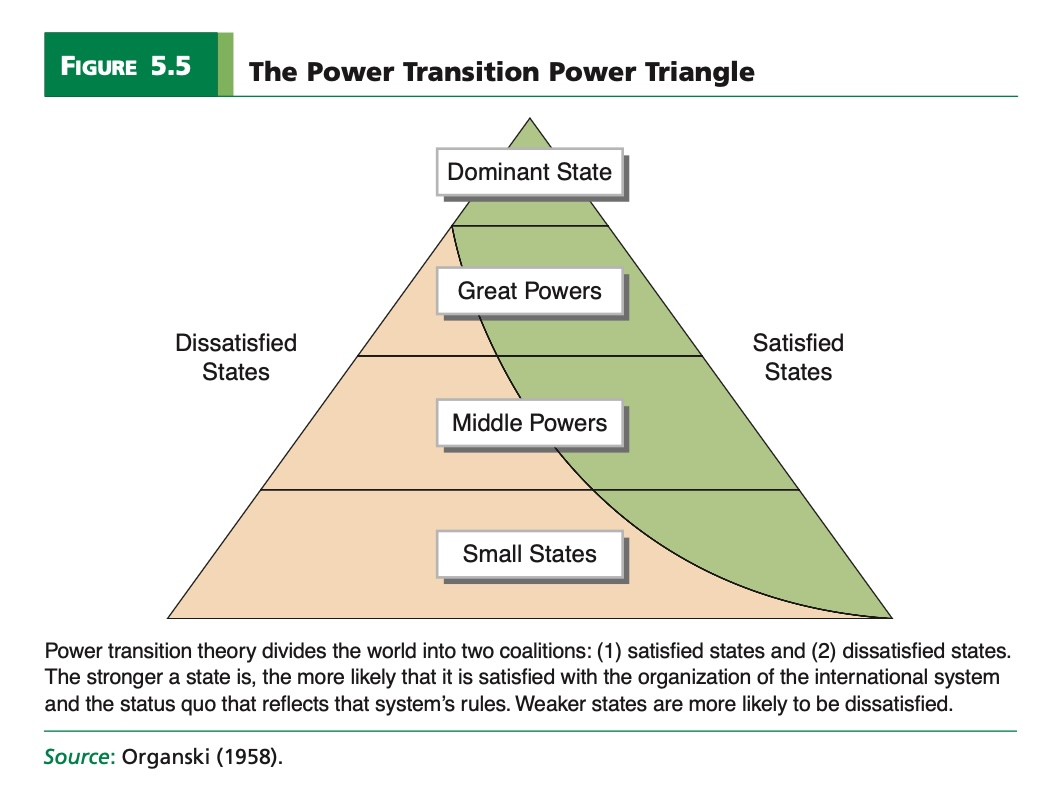
\includegraphics[width=1\textwidth]{images/power_transition_triangle.jpg}
    \captionof{figure}{\label{fig:fig1_power_transition_triangle}%\textit{\parencite[Fig.\(\backsim\)1]{cranmerWhatCanWe2017}}
    }
\end{center}

\subsection{Dissatisfaction, the Status Quo, and War}
Conflict arises when a dissatisfied state grows strong enough to challenge the authority of the hegemon. Because such a challenge concerns the very way in which international affairs are conducted, the ensuing conflict is fierce and costly.

This time period during which the challenger roughly comes to equal and then surpass the dominant state in power is known as the power transition. It is the time when the threat of a major war is hypothesized to be at its peak.
\textbf{Contrary to the balance-of-power perspective}, power transition and hegemonic stability theorists believe that major wars are most likely to occur when the power of the opposed states is about equal.

\textbf{According to these theorists, a balance of power promotes war.} They maintain that system-transforming wars—that is, wars that lead to a new power hierarchy and to new rules and norms—will occur only when the power of a challenger and the dominant state are about equal and the power of the challenger is increasing faster than that of the dominant state. These claims have been extended and shown to have \textbf{empirical strength} at the regional as well as the global level, so that regional hegemons apparently face the same pressures and the same sources of war as their global counterparts.

Threatening balance of power emerges as a result of differing rates of internal growth between a dominant state and a challenger state. These theories still give little attention to domestic politics per se, but they do recognize that internal factors shape rates of growth.

Power transition theory leads to the hypothesis that system-transforming, high-cost wars are especially likely when a dissatisfied challenger state achieves approximate power parity with the dominant, status quo-defending state.

Kim and Morrow have shown that the distribution of power at which the rivals will fight depends on their willingness to take the risks of waiting. The longer the challenger waits to attack, the higher is its probability of victory. This is true because the challenger’s power is growing faster than the dominant state’s power. Thus, the longer the challenger puts off a war, the greater will be the odds in its favor. However, the longer it waits, the longer it must endure the rules of international intercourse with which it is dissatisfied.

Kim and Morrow have shown that the interval during which the challenger is willing to fight expands as the expected costs of the war increase, as the challenger’s dissatisfaction with the status quo increases, as the challenger’s relative growth rate declines, and as the challenger becomes more risk acceptant.

How long the challenger and the dominant states will wait before fighting depends on their respective responses to risk, their relative rates of growth, the expected costs of the war, and their respective degrees of satisfaction with the status quo.

Differences in growth rates turn out not to be crucial empirically.

Power transitions per se cannot explain especially costly wars.

\begin{center}
    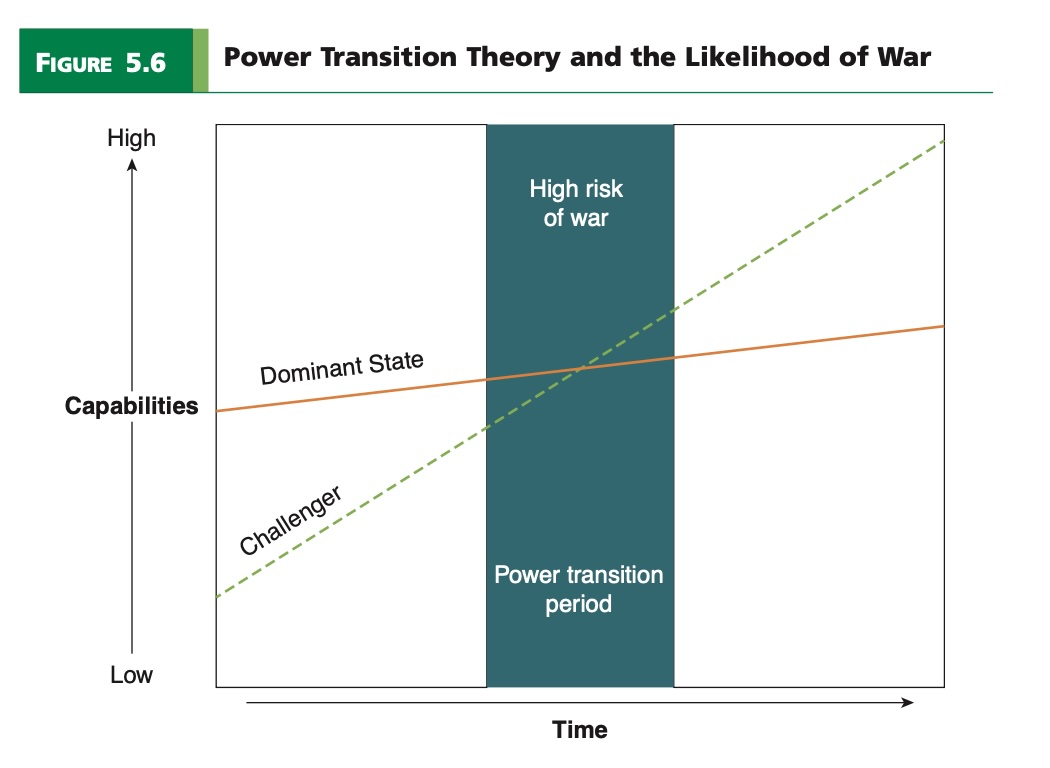
\includegraphics[width=1\textwidth]{images/power_transition_pattern.jpg}
    \captionof{figure}{\label{fig:fig1_power_transition_pattern}%\textit{\parencite[Fig.\(\backsim\)1]{cranmerWhatCanWe2017}}
    }
\end{center}

\newpage

\section{\cite{levyCAUSESWARCONDITIONS}}
This makes it hard to argue that human nature and related factors are causes of war. The point is that these factors are constants and cannot explain the variations in war and peace over time and space (Waltz 1959, Cashman 1993).

Why does war occur at some times rather than other times, between some states rather than other states, under some political leaders rather than others, in some historical and cultural contexts rather than others, and so on? This differs from still a third question: How do we explain the origins of a particular war? Most international relations scholars (and particularly those in North America) focus primarily on the second question, explaining variations in war and peace. They leave the question of why war occurs at all to philosophers and biologists and leave the question of why a particular war occurs to historians.

Although \textbf{anarchy} may provide one persuasive answer to the question of the permissive causes of war, it is generally treated as a structural constant and consequently it cannot account for variations in war and peace.

\subsection{The Levels-of-Analysis Framework}
Waltz (1959) classified the causes of war in terms of their origins in the individual, the nation-state, and the international system $\Rightarrow$ levels-of-analysis framework as an organizing device for the study of war.

In this sense the systemic level of analysis refers to explanations of patterns and outcomes in the international system; the dyadic level refers to explanations of the strategic interactions between two states; the national level refers to explanations of state foreign policy behavior; the organizational level refers to explanations of the behavior of organizations; and the individual level refers to explanations of the preferences, beliefs, or choices of individuals.

We cannot assume that correlations or causal connections at one level of analysis are necessarily valid at another level. It is conceivable, for example, that concentrations of power may promote peace at the dyadic level but war at the system level.

\subsection{Systemic-Level Theories}
The realist tradition has dominated the study of war since Thucydides and includes Machiavellians, Hobbesians, classical balance of power theorists, Waltzian neorealists, and hegemonic transition theorists. Although different realist theories often generate conflicting predictions, they share a core of common assumptions: the key actors in world politics are sovereign states that act rationally to advance their security, power, and wealth in a conflictual international system that lacks a legitimate governmental authority to regulate conflicts or enforce agreements.

\begin{itemize}
    \item they use Prisoner's Dilemma and stag-hunt models
    \item The core proposition of realist theory is that the distribution of power, throughout the system or within a dyad, is the primary factor shaping international outcomes.
\end{itemize}

We should treat realism as a paradigm rather than as a theory, and focus instead on specific theories that generate more determinant, testable propositions.

\subsubsection{Hegemonic Theory or Power Transition Theory}
Hegemonic theory is a structural theory that incorporates power transition theory and hegemonic stability theory and that \textbf{downplays the importance of anarchy}.

Hegemons commonly arise and use their strength to create a set of political and economic structures and norms of behavior that enhance the stability of the system while advancing their own security. Differential rates of growth, the costs of imperial overextension, and the development of vested domestic interests lead to the rise and fall of hegemons, and the probability of a major war is greatest at the point when the declining leader is being overtaken by the rising challenger.

Power transition theorists disagree somewhat on the precise identity of hegemonic wars and the particular causal dynamics from which they arise.

\subsubsection{Balance of Power Theory}
Balance of power theory is more concerned with explaining national strategies, the formation of blocking coalitions, the avoidance of hegemony, and the stability of the system than the origins of wars, which are underdetermined.

There is a major debate, however, between classical realists, who argue that stability is further supported by the presence of a multipolar distribution of power and a “flexible” alliance system (Morgenthau 1967, Gulick 1955), and neorealists, who argue that bipolarity is more stable than multipolarity (Waltz 1979, Mearsheimer 1990).

\textbf{Balance of power theory and power transition theory appear to be diametrically opposed}; the former argues that hegemony never occurs and that concentrations of power are destabilizing, and the latter argues the opposite.

\subsubsection{Realism and Liberalism}
The relationship between economic interdependence and war is an old question that has attracted new attention in the past few years.

\textbf{Liberal economic theory of war:} Montesquieu [1977 (1748)] stated that “peace is the natural effect of trade,” and liberal economic theorists since Smith [1937 (1776)] and Ricardo [1977 (1817)] have argued that capitalist economic systems and the free exchange of goods in an international market economy are the best guarantors of peace.

\textbf{Realist:} they often argue that the effect of trade on war is small relative to that of military and diplomatic considerations. They also question the liberal assumption that trade is always more efficient than military coercion in expanding markets and investment opportunities and in promoting state wealth.

Whether the incentives for the gains from trade dominate the incentives for coercion or protection based on economic asymmetries, and whether the latter escalate to trade wars and militarized conflicts, are empirical questions that analysts have only recently begun to analyze systematically.

\textbf{Historical and empirical evidence of trade between enemies}

Although liberals and realists disagree on the effects of trade on war, \textbf{they appear to agree that trade and other forms of economic interchange between societies will cease or be drastically reduced once states are at war with each other.} Contrary to both liberal and realist expectations, however, \textbf{there are numerous historical cases of trade between enemies} during wartime, and a preliminary quantitative study suggests that war frequently does little to depress the volume of trade between adversaries (Barbieri \& Levy 1997).

Need to incorporate domestic variables into their hypotheses

\textbf{States often hesitate to terminate trade with the enemy for fear that they will lose that trade to a third party}, who may be a greater economic or military rival.

These omissions have led all but the most committed neorealists to conclude that \textbf{systemic-level theories are theoretically incomplete and empirically inadequate}, in that \textbf{they leave too much of the variation in the outbreak and expansion of war unexplained.}


\subsection{Social-Level Theories}

Although interest in Marxist-Leninist theories has waned, there has been a tremendous growth of research on the relationships between regime type, particularly democratic regimes, and war (analyzed by Ray in this volume). Scholars have also devoted attention to the "diversionary" use of force for domestic political purposes, to the impact of ethnonationalism on international conflict, and to other domestic sources of international conflict.

"rally around the flag" effect (Mueller 1973).

This is the age-old "scapegoat hypothesis" or "diversionary theory of war" (Levy 1989a).

As Bodin argued, "the best way of preserving a state, and guaranteeing it against sedition, rebellion, and civil war is to...find an enemy against whom [the subjects] can make common cause" (quoted in Levy 1989a, p. 259).

research on the scapegoat hypothesis

The absence of significant findings regarding the relationship between internal and external conflict contrasts sharply with evidence of external scapegoating from historical and journalistic accounts and from a growing body of case-study evidence.

Most of these studies have focused on democratic regimes, partly because of the ease of measuring elite support levels but also because of the assumption that the greater political accountability of leaders in democratic states makes them more likely than authoritarian leaders to engage in external scapegoating.

These models help to explain "gambling for resurrection" through risky foreign policies by poor leaders who expect to be removed by their constituents (Downs \& Rocke 1995).

This raises the question of how external actors perceive and respond to diversionary actions.

Marxist-Leninist models of imperialism, like models of scapegoating, implicitly assume that external expansion and the use of force serve the interests of the ruling class or elite but not those of society as a whole.

If the costs of aggressive foreign policies are too high---and we have enough examples of "imperial overstretch" to suggest that they sometimes are---it is not clear how elites maintain their power. As Snyder (1991) argued, groups concentrated enough to benefit from overexpansion are too narrow to control state policy, while those broad enough to control policy are too diffuse to reap benefits from overexpansionist policies.

For Snyder, this rationalist model of logrolling is not sufficient to explain overexpansion or the stability of the ruling coalition.

\subsection{Individual-Level Theories}
decision-making is characterized by “bounded rationality”
\textbf{Assumptions:}
\begin{enumerate}
    \item [(a)] that external and internal structures and social forces are not translated directly into foreign policy choices;
    \item [(b)] that key decision-makers vary in their definitions of state interests, assessments of threats to those interests, and/or beliefs as to the optimum strategies to achieve those interests; and
    \item [(c)] that differences in the content of actors’ belief systems, in the psychological processes through which they acquire information and make judgments and decisions, and in their personalities and emotional states are important intervening variables in explaining observed variation in state behaviors with respect to issues of war and peace.
\end{enumerate}

\textbf{Prospect Theory} one of the most recent attempts to apply a social-psychological model to international relations (Kahneman \& Tversky (1979)).

Prospect theory assumes that people evaluate outcomes in terms of deviations from a reference point or aspiration level rather than in terms of net-asset levels.

This asymmetry of behavior with respect to gains and losses means that the way people frame their reference point in any given choice problem is critical.

\subsection{General Trends}

\begin{itemize}
    \item shift away from the systemic level: dissatisfaction with the failure of structural systemic models to explain enough of the variance in war and peace. This shift has led to rising interest in both dyadic-level behavior and societal-level explanatory variables.
    \item Whatever the relationship between concentrations of military and economic capabilities at the systemic level, there is substantial evidence that at the dyadic level an equality of capabilities is significantly more likely to lead to war.
    \item In the past decade most international relations theorists have moved beyond their earlier preoccupation with explanations at a single level of analysis and debates about which level provides the most powerful explanations. They now give much more attention to interaction effects among variables at different levels in the processes leading to war
\end{itemize}


\section{One World Rival Theories}
\textcite{snyderOneWorldRival2004}

\begin{center}
    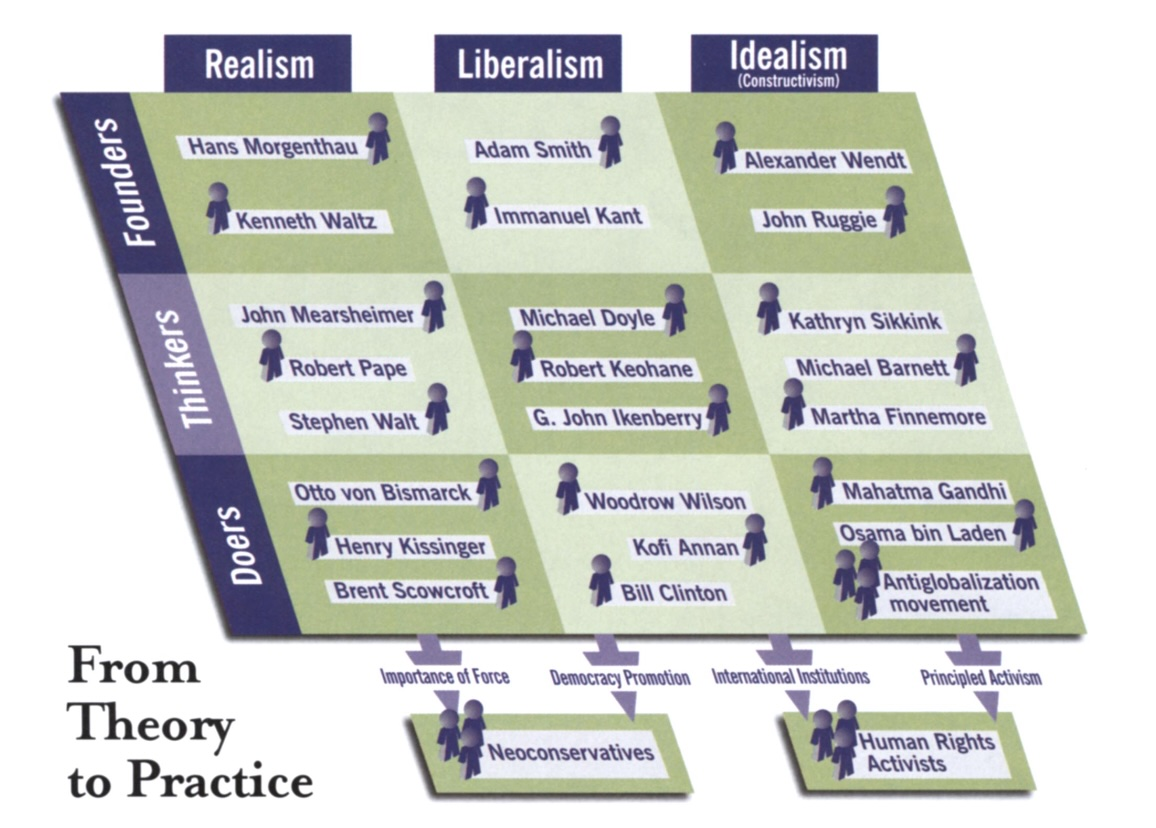
\includegraphics[width=0.7\textwidth]{images/snyder_one_world_rival_theories.jpg}
    \captionof{figure}{\label{fig:fig4_snyder_one_world_rival_theories}%\textit{\parencite[Fig.\(\backsim\)1]{cranmerWhatCanWe2017}}
    }
\end{center}

Realism instills a pragmatic appreciation of the role of power but also warns that states will suffer if they overreach. Liberalism highlights the cooperative potential of mature democracies, especially when working together through effective institutions, but it also notes democracies' tendency to crusade against tyrannies and the propensity of emerging democracies to collapse into violent ethnic turmoil.

Idealism stresses that a consensus on values must underpin any stable political order, yet it also recognizes that forging such a consensus often requires an ideological struggle with the potential for conflict.

It is harder for the normally state-centric realists to explain why the world’s only superpower announced a war against al Qaeda, a nonstate terrorist organization. How can realist theory account for the importance of powerful and violent individuals in a world of states? Realists point out that the

Post-9/11 developments seem to undercut one of realism's core concepts: the balance of power.

When Germany unified in the late 19th century and became Europe's leading military and industrial power, Russia and France (and later, Britain) soon aligned to counter its power. Yet no combination of states or other powers can challenge the United States militarily, and no balancing coalition is imminent.

\subsection{The Divided House of Liberalism}
For its part, the Bush administration highlights democracy promotion while largely turning its back on the international institutions that most liberal theorists champion.

The belief that democracies never fight wars against each other is the closest thing we have to an iron law in social science.

Shortly before September 11, political scientist G. John Ikenberry studied attempts to establish international order by the victors of hegemonic struggles in 1815, 1919, 1945, and 1989. He argued that even the most powerful victor needed to gain the willing cooperation of the vanquished and other weak states by offering a mutually attractive bargain, codified in an international constitutional order.

\begin{center}
    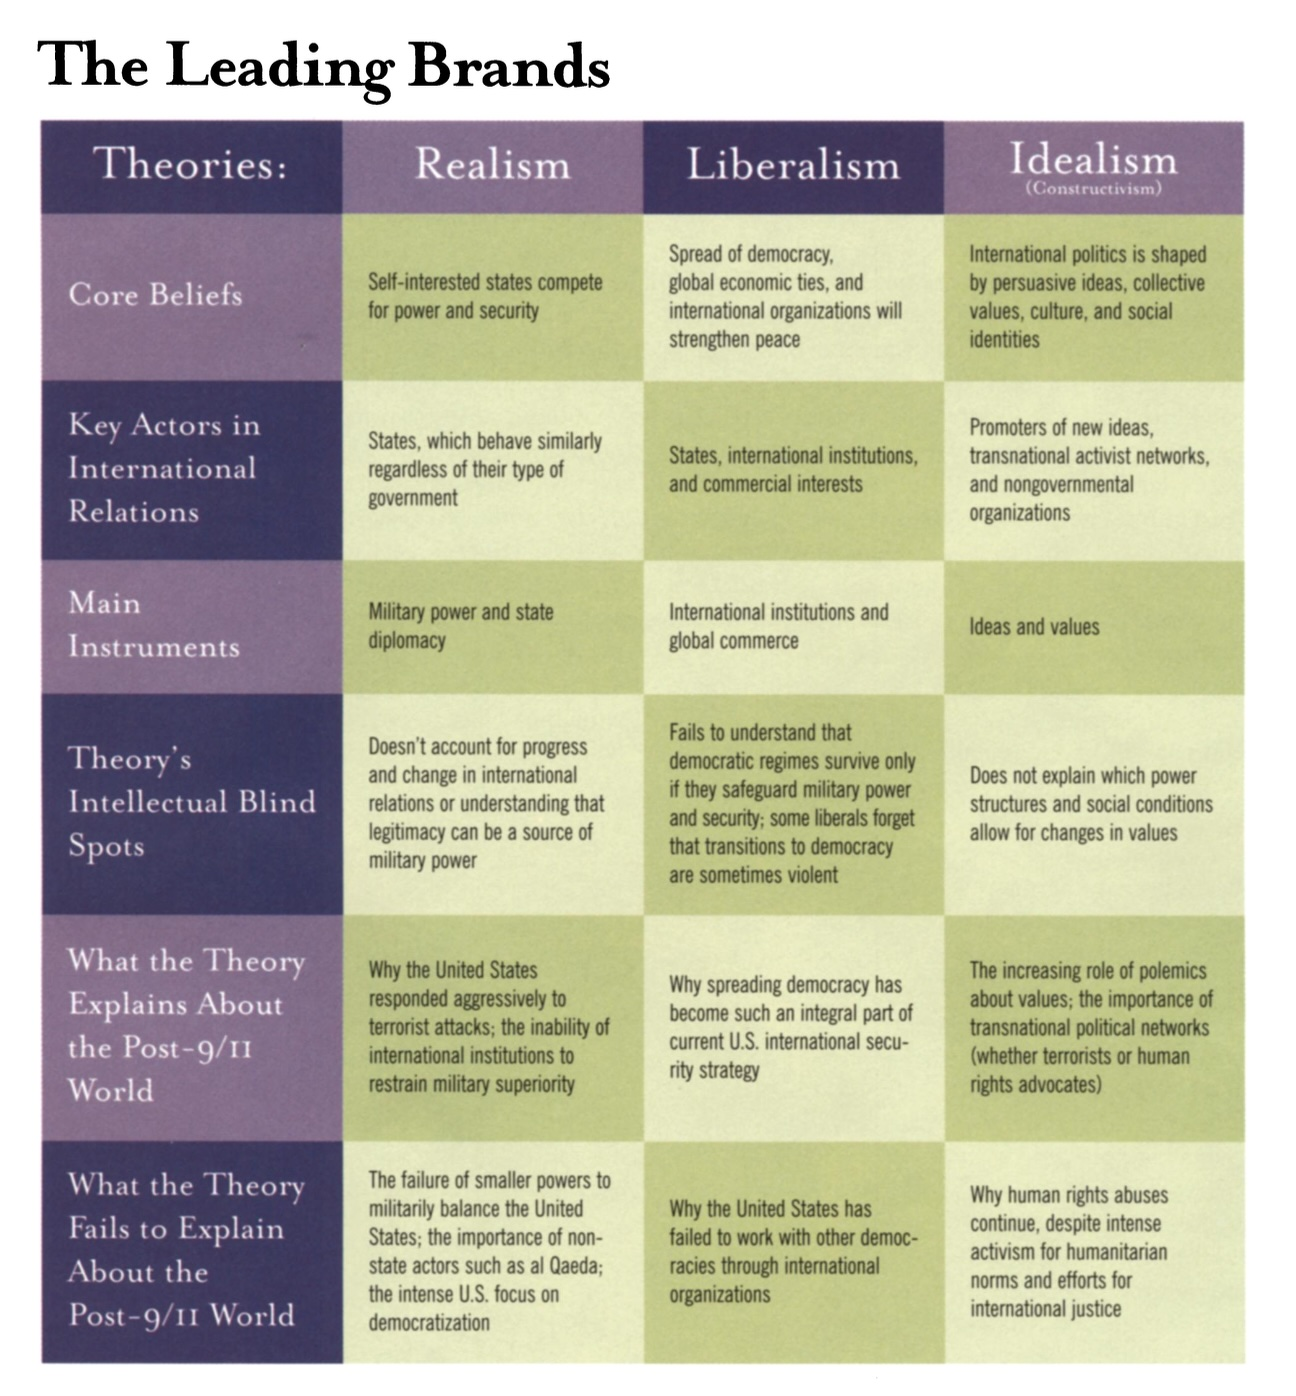
\includegraphics[width=0.7\textwidth]{images/snyder_one_world_rival_theories_the_leading_brands.jpg}
    \captionof{figure}{\label{fig:fig5_snyder_one_world_rival_theories_the_leading_brands}%\textit{\parencite[Fig.\(\backsim\)1]{cranmerWhatCanWe2017}}
    }
\end{center}

\subsection{Idealism}
Idealism: the belief that foreign policy is and should be guided by ethical and legal standards.

\textbf{Constructivism is a new version of idealism:} holds that social reality is created through debate about values, often echoes the themes that human rights and international justice activists sound.

Perhaps most important, Europe’s increasingly legalistic approach to international relations, reflected in the process of forming the European Union out of a collection of sovereign states, provides fertile soil for idealist and constructivist conceptions of international politics.

\textbf{Whereas realists dwell on the balance of power and liberals on the power of international trade and democracy, constructivists believe that debates about ideas are the fundamental building blocks of international life. Individuals and groups become powerful if they can convince others to adopt their ideas.}

Realists failed to predict the end of the Cold War, for example. Even after it happened, they tended to assume that the new system would become multipolar.

Likewise, the liberal theory of democratic peace is stronger on what happens after states become democratic than in predicting the timing of democratic transitions, let alone prescribing how to make transitions happen peacefully.

Constructivists are good at describing changes in norms and ideas, but they are weak on the material and institutional circumstances necessary to support the emergence of consensus about new values and ideas.

With such uncertain guidance from the theoretical realm, it is no wonder that policymakers, activists, and public commentators fall prey to simplistic or wishful thinking about how to effect change.


% !TEX root = ./main.tex
% Summary of David A. Lake (2011), "Why \"isms\" Are Evil"
% This file is intentionally a LaTeX fragment: it does not load a document class
% or packages, so it can be included from your existing main.tex/sty setup.

\section{Why "isms" Are Evil David Lake}
\cite{lakeWhyIsmsAre2011}



\subsection{Central Argument and
Purpose}

Lake's essay is a critique of how international studies is organized
intellectually and professionally. His central claim is not that
theoretical diversity is undesirable, but that scholars have turned
theoretical traditions and epistemological preferences into academic
``sects.'' Instead of using theories as limited tools for understanding
specific problems, researchers often treat broad traditions such as
realism, liberalism, constructivism, Marxism, neoliberal
institutionalism, feminism, or the English School as competing
intellectual religions. Each group tends to defend its own assumptions,
produce research that confirms those assumptions, and debate rival
traditions at the level of first principles. In Lake's view, this
sectarian organization generates less understanding rather than more. It
also distracts scholars from their fundamental social responsibility:
improving knowledge of world politics and, where possible, identifying
ways to promote more humane outcomes.

The problem is especially serious because the discipline does not
possess a single, universal and empirically powerful theory of
international politics. World politics is too complex, and existing
knowledge is too incomplete, for one general framework to explain
everything. Lake therefore urges intellectual humility. Scholars should
accept that most theories are partial and contingent, specify the
conditions under which they apply, and concentrate on mid-level
explanations of concrete phenomena. He favors ``analytic eclecticism'':
researchers should be willing to draw on different assumptions and
theories when different problems require different tools. At the
epistemological level, he makes a parallel argument. The divide between
nomological and narrative forms of explanation is real and enduring, but
neither approach is universally superior. Both can produce valid
knowledge, and the relevant question is which approach is most
illuminating for a particular research problem.

\subsection{Theory: How Research Traditions Become Academic
Sects}

International studies has long been divided into what are often called
paradigms, but Lake prefers the term ``research traditions.'' Each
tradition contains a set of core assumptions concerning the relevant
actors in world politics, their interests, the processes through which
they make decisions, and the nature of political interaction. Different
traditions may focus on individuals, groups, states, or other
collectivities; assume that actors seek wealth, power, security, status,
identity, or justice; and portray international politics as
fundamentally conflictual, cooperative, or socially constructed. These
assumptions are useful because they simplify a complex reality and help
researchers identify puzzles. The difficulty arises when scholars forget
that they are simplifications and begin to treat them as complete
theories or even as truths about the world.

Lake argues that the coexistence of many traditions should be expected.
International politics is an exceptionally complicated social system, so
it is unsurprising that different approaches illuminate different parts
of it. The discipline's weakness lies not in pluralism itself but in the
professional practices that transform pluralism into sectarianism. He
identifies five linked pathologies. Together they encourage scholars to
defend approaches rather than explain phenomena, reward intellectual
extremism, and create self-confirming research communities.

\subsection{The first pathology: reifying research
traditions}

The first pathology is the reification of research traditions. Scholars
routinely organize literature reviews, courses, graduate seminars,
handbooks, and disciplinary histories around familiar ``isms.'' This has
practical advantages because it provides a convenient map of a large
literature, but it also creates artificial boundaries. Complex
scholarship is reduced to a few recognizable schools, subtle differences
within traditions disappear, and authors are classified according to
labels they may not accept themselves. Scholars may see their own work
as eclectic and nuanced while categorizing opponents as ``realists,''
``constructivists,'' or ``liberals.'' As a result, intellectual
identities are partly imposed by others. The discipline collectively
produces the very categories that then appear to be natural and
independent objects.

\subsection{The second pathology: rewarding
extremism}

Once research traditions are reified, the discipline rewards the
clearest and most extreme statements of each tradition. Canonical works
such as Waltz's Theory of International Politics, Keohane's After
Hegemony, or Wendt's Social Theory of International Relations become
shorthand for entire approaches. In the process, qualifications and
subtleties are often lost. These iconic texts gain visibility through
citations and teaching, while younger scholars learn that professional
recognition may come from taking a distinctive sectarian position. New
``isms'' and specialized sections of professional associations can also
become vehicles for status and intellectual entrepreneurship. The result
is a centrifugal process in which extremism generates more extremism,
even if the original authors were more nuanced than later portrayals
suggest.

\subsection{The third pathology: confusing traditions with
theories}

The third pathology is the tendency to mistake a research tradition for
a complete theory. A tradition usually supplies broad assumptions, but
those assumptions are rarely sufficient to generate unique, deductively
valid predictions. Lake uses neorealism as an example. Waltz claimed
that anarchy and the desire for survival imply balancing behavior, yet
the same assumptions can also be compatible with cooperation, collective
security, or bandwagoning unless additional assumptions are introduced.
Similar indeterminacy appears in debates over relative versus absolute
gains in neorealism and neoliberalism. This is why several distinct
theories can coexist inside a single tradition---for example, offensive
realism, defensive realism, and neoclassical realism. They share some
core premises but differ in auxiliary assumptions. Because traditions
are often underspecified, they cannot be meaningfully ``tested'' as
wholes. Yet scholars frequently stage empirical contests between
traditions as if each generated clear predictions, producing debates in
which each side can interpret evidence as confirmation.

\subsection{The fourth pathology: selective empirical
focus}

The fourth pathology is empirical selectivity. Researchers tend to study
the topics, periods, and cases in which their preferred tradition is
most likely to perform well. Realists often focus on great-power
security, liberals on economic policy, institutionalists on
institutions, constructivists on norm change, and English School
scholars on socialization and international society. This pattern need
not result from deliberate bias; it can emerge naturally because
scholars test theories where they initially expect them to work, while
journals and publishers also favor positive findings. Nevertheless, the
cumulative consequence is self-confirmation. Each tradition studies its
strongest domain, finds supportive evidence, and then treats that
evidence as proof of general explanatory power. The research tradition
begins to function like theology: evidence is selected to affirm a prior
commitment rather than used to subject theory to demanding attempts at
falsification.

\subsection{The fifth pathology: the search for intellectual
hegemony}

The fifth pathology is the aspiration of each research tradition to
become the dominant scientific paradigm. Scholars often identify
themselves as realists, constructivists, or institutionalists in ways
that imply their preferred approach is broadly superior to alternatives.
Professional incentives reinforce this competition. If a tradition
becomes dominant, its leading scholars gain status, influence, and
control over disciplinary agendas. Because every group fears losing
ground to its rivals, competition for hegemony resembles an arms race:
even scholars who would prefer cooperation feel pressure to defend and
expand their approach. The collective result is worse for everyone.
Rather than acknowledging the limited scope of existing theories,
research communities expend enormous energy debating assumptions such as
whether actors are rational, whether structure or agency matters more,
or whether power, wealth, norms, or identity should be treated as
fundamental. Without comparable theories applied to the same phenomena,
these ``first-principle'' debates cannot be decisively resolved.

\subsection{Lake's Alternative: Problems, Partial Theories, and a Common
Lexicon}

Lake's preferred alternative is to reorganize scholarship around
substantive problems rather than around intellectual sects. Courses,
conference sections, and research agendas could focus on issues such as
war, climate change, development, inequality, genocide, or political
violence. The guiding question would then be ``What do we know about
this problem?'' rather than ``What are the core assumptions of this
school?'' Such an organization would encourage scholars to compare
explanations on the basis of their contribution to understanding a
phenomenon instead of their loyalty to a tradition.

A central part of this alternative is what Lake calls an ``embrace of
partiality.'' Theories should state their scope and boundary conditions
explicitly and identify what they do not explain. A theory is not
weakened merely because it applies only under certain conditions. On the
contrary, clarity about limits improves scientific evaluation because
scholars can distinguish genuine failures from cases outside a theory's
intended domain. Lake proposes that authors should routinely include a
brief statement of boundary conditions and explanatory limitations. This
would also make it easier to combine knowledge from different theories.
His metaphor is the familiar image of several people touching different
parts of an elephant: each theory may capture one part accurately, while
no single theory describes the entire animal.

Lake explicitly rejects atheoretical research. Theories remain necessary
for explaining patterns and identifying causes. His argument is instead
that scholars should use theories flexibly. A researcher might employ a
rational unitary-state model to study war, a theory of individual norms
to investigate global environmental change, and a sectoral
material-interest model to explain trade policy. Using different
theories for different problems should not be treated as intellectual
inconsistency if each theory is appropriate to the question at hand.

\subsection{Interests, interactions, and institutions as a ``Rosetta
stone''}

Analytic eclecticism creates a possible communication problem: if
scholars abandon fixed traditions, the field could become a ``tower of
Babel'' in which theories are too different to compare. Lake therefore
proposes a common lexicon built around three broad concepts: interests,
interactions, and institutions. Any complete theory of politics must
specify who the relevant actors are, what they want, how they interact,
and the institutional environment in which interaction occurs. Actors
may be individuals, groups, organizations, or states. Interests may
involve power, wealth, identity, status, security, or normative goals.
Interactions may involve zero-sum bargaining, cooperation,
socialization, or the reproduction of inequality. Institutions may range
from weak or epiphenomenal arrangements to dense structures that
constitute actors and enable communication itself.

This lexicon is deliberately neutral among traditions. A rationalist
theory may assume groups pursue material interests, while a
constructivist theory may explain interests as socially constituted. A
realist analysis may treat states as the principal actors, while another
approach disaggregates states into domestic groups. Yet both can still
be translated into the same basic questions about actors, interests,
interactions, and institutions. Components can also be modular:
something treated as given in one theory can be explained in another.
Regime type, for example, may be used as an independent variable in a
theory of war and then become the dependent variable in a separate
theory of democratization. The goal is not theoretical unification, but
clearer comparison, better specification, and cumulative knowledge.

\subsection{Epistemology: The Enduring
Divide}

Lake then turns from theory to epistemology. He identifies a deep divide
between nomological and narrative forms of explanation. This cleavage
has shaped major debates in international relations for decades and, in
his view, is harder to bridge than differences among theoretical
traditions. However, he does not believe that one epistemology will or
should defeat the other. Both have long histories, both respond to
different intellectual intuitions, and both can generate valuable
knowledge. The discipline should therefore accept epistemological
diversity rather than politicize it.

\subsection{The nomological approach}

The nomological approach seeks generalizable explanations based on
covering laws or theoretically specified relationships. It typically
uses the hypothetical-deductive method: researchers derive falsifiable
propositions of the form ``if X, then Y'' and test them using designs
that approximate controlled experiments. True experiments offer the
strongest internal validity, followed by quasi-experiments and then
correlational studies such as regression analysis. Causal claims can
emerge either from a strong design that isolates the effect of X on Y or
from a combination of theory and robust empirical association. Lake
notes that much international-relations research relies on the weaker
correlational form. Science in this tradition is iterative: theory
generates hypotheses, evidence tests them, and theories are revised,
extended, or occasionally rejected.

For Lake, generalizability in nomological research depends primarily on
theory rather than on the particular sample used in a test. If a theory
is explicitly intended to apply to all humans, evidence from a narrower
sample can still be relevant provided the test has strong internal
validity. Conversely, findings from a particular population cannot
validate a theory whose assumptions do not extend to that population.
External validity therefore rests on clearly specified scope and
boundary conditions.

\subsection{The narrative approach}

The narrative protocol organizes explanation differently. It begins with
a descriptive order that links events through time and examines how each
development shapes what follows. It then constructs a configurative
order by adjusting an interpretive framework to the historical facts
through a process of abduction. The objective is to produce a convincing
and plausible account of why events unfolded as they did. Narrative
explanations are often richer and more holistic than nomological models
because they emphasize combinations of causes and historically specific
conjunctures. Their weakness, in Lake's view, is that the criteria for
judging causal adequacy are more subjective. Narratives are evaluated in
terms of verisimilitude and interpretive credibility rather than
experimental internal validity.

Lake stresses that epistemology should not be confused with methodology.
A nomological study can use historical case studies and process tracing,
while a narrative analysis can employ large numbers of observations or
statistical techniques. ``Mixed methods'' can improve research by
testing theories in multiple ways, but mixing methods does not by itself
eliminate the distinction between forms of explanation. Method concerns
the techniques used to gather and analyze evidence; epistemology
concerns what counts as a persuasive explanation.

\subsection{Epistemological Sectarianism and Lake's
Recommendations}

The same pathologies that affect theory also affect epistemology.
Scholars reify the nomological and narrative approaches, reward extreme
positions, apply them selectively to problems where they are likely to
succeed, and then claim universal superiority. These preferences have
become politicized within the profession. Epistemological gatekeepers
can influence hiring, resource allocation, publication, and access to
professional networks, encouraging scholars to cluster with others who
share the same standards of explanation. Lake sees no objective basis
for declaring one epistemology universally superior. Scholars may simply
find one form of explanation more intuitively satisfying than another,
much as some people find beauty in mathematics and others in poetry.

Because neither epistemological tradition is likely to eliminate the
other, Lake proposes three principles for coexistence. First, scholars
should recognize the legitimacy of alternative forms of explanation and
respect colleagues who use them. Treating one's own epistemological
intuition as inherently superior is a form of intellectual hubris.
Second, each approach should be judged on its own terms. Narrative work
should be assessed for completeness, plausibility, competing
interpretations, and possible distortion of historical evidence.
Nomological work should be evaluated for logical deduction, valid
operationalization, and sound research design. Third, scholars should
accept that different approaches are likely to work better for different
questions.

Lake illustrates this final point with substantive examples. Narrative
approaches may be especially effective for slow, historically unique
changes in global norms, such as transformations in attitudes toward
slavery or human rights. Such processes unfold over long periods and are
difficult to analyze while holding the social environment constant. By
contrast, nomological approaches may be especially powerful when
interactions are frequent and institutions are stable enough to generate
repeated observations. Research on war and civil war, or on economic
policymaking within established democratic institutions, can often
benefit from this kind of analysis. The crucial question is therefore
not ``Which epistemology is best?'' but ``Which epistemology provides
the greatest insight for this particular problem?''

\subsection{Conclusion}

Lake concludes by returning to the social purpose of scholarship.
Academic privilege is justified by the expectation that scholars will
expand understanding. International studies fails in this responsibility
when it devotes too much energy to theological wars among theoretical
and epistemological camps. Progress comes from asking important
questions about phenomena that remain poorly understood, choosing
theories and methods appropriate to those questions, and evaluating
evidence honestly. At the present stage of the discipline, no
theoretical or epistemological approach merits hegemony. Diversity is
necessary, but diversity should not take the form of isolated
communities that speak mainly to themselves.

The essay's title is therefore deliberately provocative. ``Isms'' are
``evil'' not because realism, liberalism, constructivism, feminism, or
other traditions are useless, but because scholars too often transform
useful intellectual tools into identities and sects. Research traditions
become harmful when they are treated as complete theories, insulated by
selective evidence, and mobilized in struggles for disciplinary
dominance. Lake's alternative is a more modest and problem-centered
social science: partial theories with explicit limits, analytic
eclecticism across traditions, a shared vocabulary of interests,
interactions, and institutions, and mutual respect between nomological
and narrative forms of explanation. The ultimate measure of success
should be whether scholarship improves our understanding of world
politics and contributes, where possible, to social progress.


\section{Challenges to the Liberal Order: Summary}
\begin{center}
\textit{David A. Lake, Lisa L. Martin, and Thomas Risse (2021)}
\end{center}

\subsection{Introduction and Central Argument}

The Liberal International Order (LIO) is under pressure from several directions at once. The authors emphasize that the postwar order has survived serious crises before, so its collapse should not be assumed.

The LIO has structured relations among the capitalist, democratic, and industrialized states since the late 1940s and has had wider global effects. It is associated with unprecedented cooperation among North America, Western Europe, and Japan, the emergence of a pluralistic security community, expansion of trade and capital mobility, high economic growth, the diffusion of democracy, and the development of an international human-rights regime.

\subsection{Order}

An order consists of patterned or structured relations. The LIO is clearly rule-governed and sustained by coordinated action by both state and nonstate actors.

\subsection{International and the Westphalian Order}

The "international" component of the LIO has to be understood in relation to the Westphalian order. In the authors' usage, Westphalia is not literally a system created in 1648 but a later order centered on sovereign nation-states, sovereign equality, recognition by other states, and noninterference in domestic affairs. The LIO and the Westphalian order partly overlap and have coevolved since 1945. They share principles such as sovereign equality, peaceful settlement of disputes, self-determination, and nonintervention. At the same time, the LIO goes beyond Westphalia through principles such as human rights and forms of legitimate collective intrusion into domestic affairs.

\begin{center}
    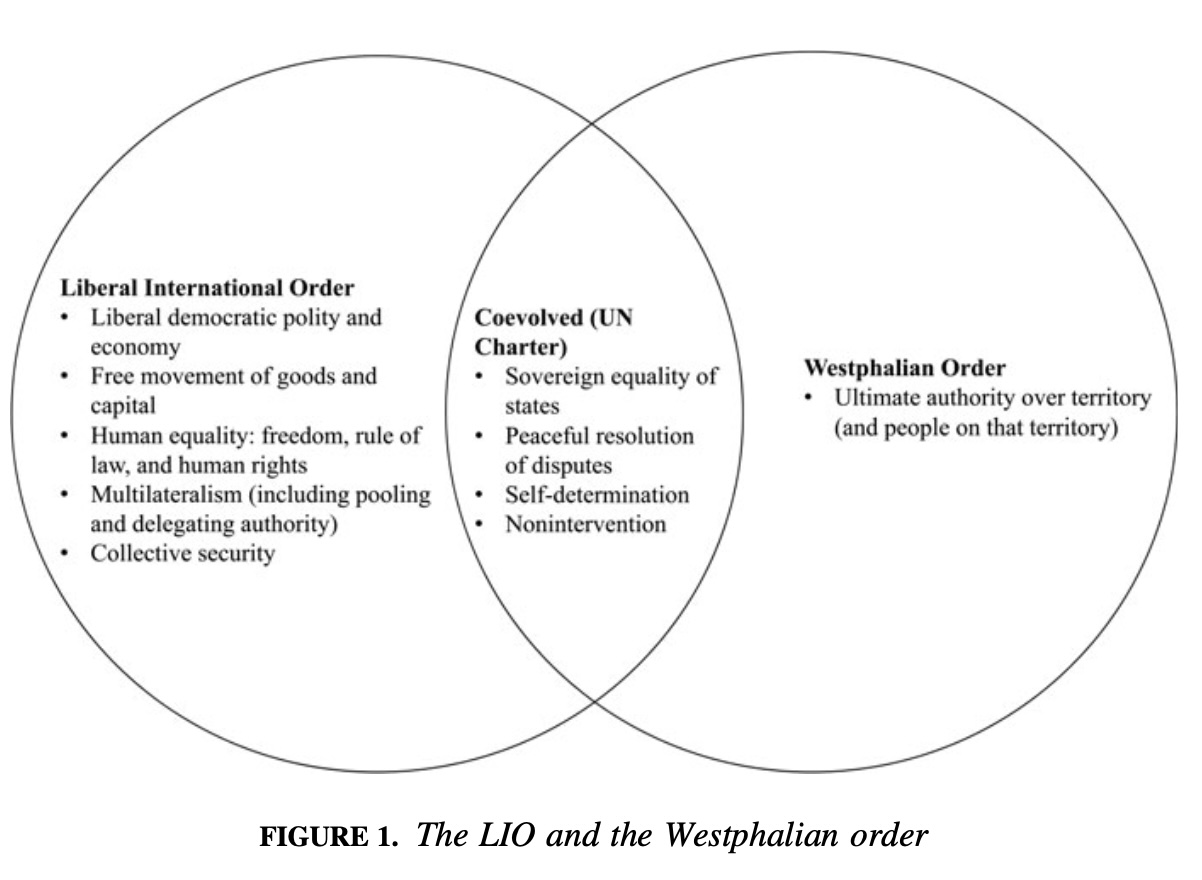
\includegraphics[width=1\textwidth]{images/challenges_to_liberal_order_LIO_vs_westphalian.jpg}
    \captionof{figure}{\label{fig:fig6_challenges_to_liberal_order_LIO_vs_westphalian.jpg}%\textit{\parencite[Fig.\(\backsim\)1]{cranmerWhatCanWe2017}}
    }
\end{center}

\subsection{Liberal: Political Liberalism}
At its philosophical core, liberalism rests on universal human equality, freedom, and individual and collective self-determination. Political liberalism therefore implies the rule of law, representative government, political participation, and protection of individual rights.

Institutions such as the International Criminal Court and doctrines such as the Responsibility to Protect illustrate how the LIO can authorize constraints on domestic sovereignty in the name of universal rights.

\subsection{Economic Liberalism and Embedded Liberalism}

A classical version favors market capitalism, free trade, international capital mobility, and equal treatment of foreign investment.

A second, historically important version is embedded liberalism. The postwar architects of the Bretton Woods system combined trade liberalization with domestic welfare states.

The distinction is important because economic liberalism does not automatically contradict Westphalian sovereignty.

The LIO broadly liberalized goods, services, and capital but never generally established free movement of labor outside the EU.

\subsection{Liberal Internationalism}

The institutional dimension of the LIO is based on principled multilateralism. Multilateralism means more than coordination among several states: it means coordination according to generalized rules that apply across cases rather than ad hoc bargaining based solely on particular interests. The GATT,WTO and UN Charter exemplify this logic. Liberal internationalism also includes peaceful dispute resolution, the ambition to provide global public goods, security communities such as NATO, and multilateral arms-control and nonproliferation regimes.

\textbf{Tensions with Westphalia:}
\begin{enumerate}
    \item Authority is delegated supranational bodies
    \item Majority voting
    \item Dispute-settlement mechanisms
    \item International courts.
\end{enumerate}

\subsection{Universalism and Selective Participation}

The LIO contains a paradox. Because liberalism begins from universal equality, the order is in principle open to all states. Yet states can join important parts of the LIO without being liberal democracies.

The LIO is therefore best understood as an evolving order whose components vary in reach rather than as a single uniform system imposed everywhere by the United States.

\subsection{Challenges from Within the Liberal Core}

The most striking contemporary threats come not only from geopolitical rivals but also from the internal workings of liberalism itself. The authors identify several mechanisms through which the LIO generates opposition within its own core members.

\begin{enumerate}
    \item Economic liberalism creates winners and losers. Trade openness, technological change, global production chains, and the financial crisis of 2008--2010 have produced geographically concentrated losses and contributed to rising inequality.
    \item Political openness can be used against liberalism. Freedom of expression and the open architecture of the internet allow misinformation, foreign influence, and strategies of "truth subversion" to circulate widely. 
    \item Free-trade policies and supranational governance were sometimes insulated from popular pressure in order to prevent protectionism and secure long-term cooperation. Over time, however, this technocratic insulation excluded some constituencies and created resentment. International institutions appeared less responsive to citizens.
    \item liberal universalism collides with national identity. Who belongs to the national community? Migration is a problem
\end{enumerate}

\subsection{Nationalist Populism and Political Realignment}

These pressures converge in movements combining nationalism, populism, and authoritarianism. Nationalism prioritizes the interests and identity of a particular state; populism pits a supposedly homogeneous "people" against elites and pluralist institutions; authoritarianism rejects liberal constraints such as independent courts, a free press, and fair electoral competition.

\subsection{External Challengers}

\begin{itemize}
    \item Climate change
    \item Distributional conflicts due to Climate change
    \item China: Its extraordinary economic growth was enabled by participation in the open international economy, yet China remains authoritarian and strongly defends sovereignty and noninterference.
\end{itemize}

\subsection{The Erosion of Multilateral Institutions}

Internal and external challenges converge most directly in attacks on multilateralism. Multilateral institutions have experienced crises before, including the collapse of the Bretton Woods monetary system and the US decision to invade Iraq without broad UN support. What appears different in the contemporary period is the breadth of skepticism and the willingness of major states to weaken institutions without a clear systemic necessity.

\begin{enumerate}
    \item WTO crisis: Even before the recent crisis it struggled to negotiate large new trade agreements. The United States combined protectionist tariffs with a strategy of blocking appointments to the WTO Appellate Body, impairing enforcement.
    \item Refugee crisis: The refugee regime illustrates a broader erosion of multilateral commitments. The principle of nonrefoulement and the 1951 Refugee Convention created legal obligations toward asylum seekers, yet receiving states have increasingly adopted restrictive or deterrent policies.
\end{enumerate}

\subsection{Sources of Resilience}

\begin{enumerate}
    \item the order has produced substantial benefits: reduced conflict among core members, economic growth, lower global poverty, and extensive international cooperation.
    \item LIO has generated vested interests: Firms have built global investments and supply chains that depend on open trade and predictable international rules. The same interdependence that creates vulnerability can also reinforce support for openness.
    \item the LIO institutions can outlast the circumstances that produced them and act as shock absorbers during crises.
    \item \textbf{Legitimacy}: After decades of operation, many rules of multilateral cooperation have acquired a sense of normality and rightfulness. Practices that once required active justification can become taken for granted as normal components of international life.
    
    \textbf{Accumulated normative capital}
    
    \textbf{Political baseline}
\end{enumerate}

\subsection{Four Analytic Blind Spots in IR Scholarship}

\begin{enumerate}
    \item \textbf{Exclusion}, stigma, and the threat of losing membership help enforce order. Exclusion is not merely a defect at the margins of the LIO.
    \item \textbf{Orders Are Not Neutral:} distributional consequences and the fact that rules are written by particular actors for particular purposes. Cooperation can be Pareto-improving while still distributing gains unequally.
    \item \textbf{Institutions Depend on Social Foundations:} Institutions survive because social groups invest political resources in creating and defending them. Institutional insulation may sometimes be necessary to protect long-term cooperation from short-term pressures.
    \item \textbf{Domestic Politics Can Challenge the Order Itself:} IR scholarship  paid little attention to the possibility that parties, protest movements, territorial cleavages, and mass political realignments inside core states could attack the international order itself.
\end{enumerate}

\subsection{USA and the Future of LIO}
Question about American leadership.

\begin{itemize}
    \item The LIO could survive because existing institutions and old and new stakeholders defend it.
    \item more traditional Westphalian order centered on sovereignty and noninterference.
    \item It could be transformed into a hybrid order that preserves economic openness and principled multilateralism while altering commitments to democracy, human rights, and international legal authority.
\end{itemize}

\newpage
\part{Session 3}
\textbf{Session 3, February 23: The strategic perspective}

\begin{itemize}
    \item [***] \textcite[Introduction]{cranmerWhatCanWe2017}
    \item \textcite[Chapter 1]{cranmerWhatCanWe2017}
    \item \textcite[Chapter 2]{cranmerWhatCanWe2017}
\end{itemize}

% \begin{center}
%     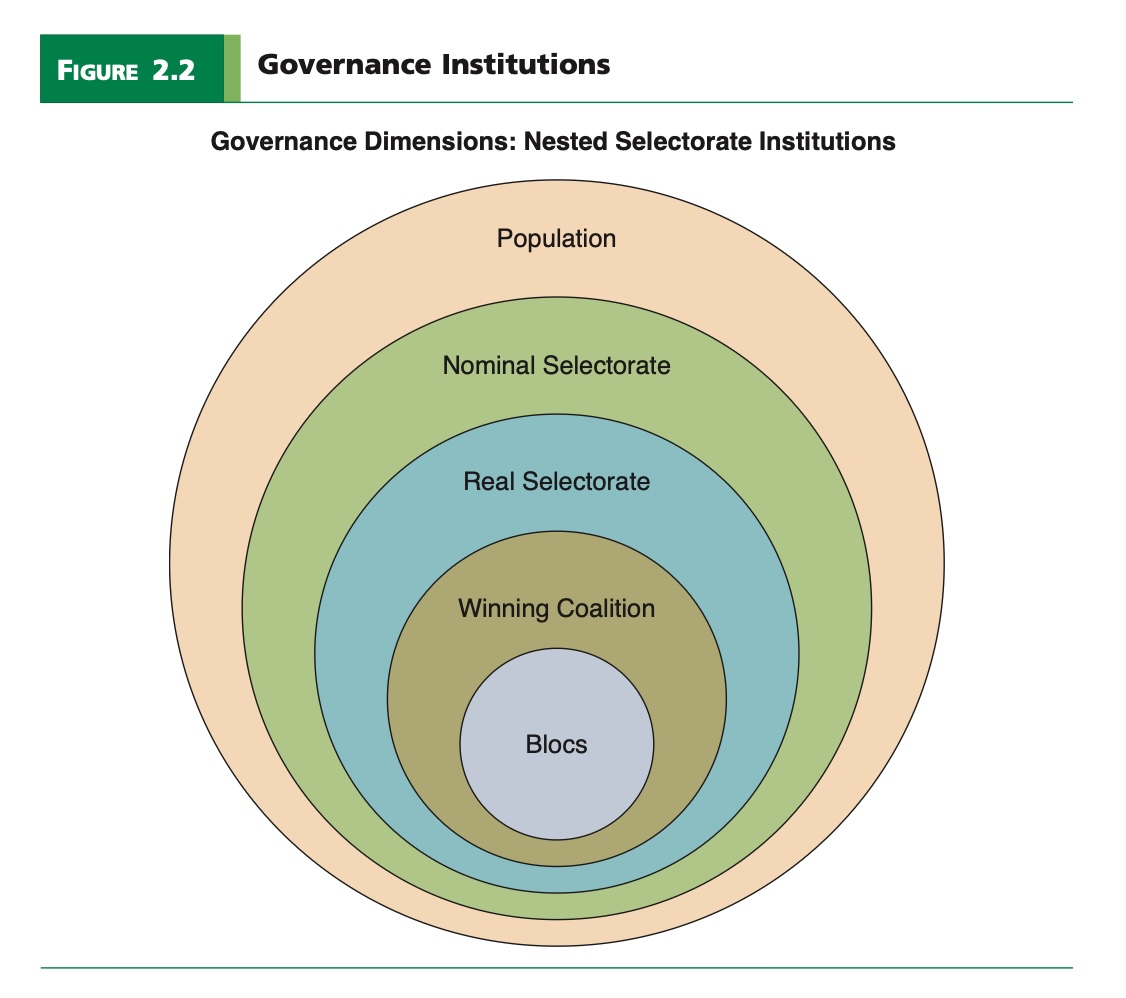
\includegraphics[width=0.7\textwidth]{images/nested_selectorate_institutions.jpg}
%     \captionof{figure}{\label{fig:fig3_nested_selectorate_institutions}%\textit{\parencite[Fig.\(\backsim\)1]{cranmerWhatCanWe2017}}
%     }
% \end{center}

\section{Semantic Role Labelling}


\subsection{SELECTORATE THEORY}
The selectorate theory represents one version of the strategic perspective.

In selectorate theory, leaders build a coalition of supporters among the selectorate. The selectorate (S) consists of those who have at least a nominal say in choosing leaders and are eligible to become members of a winning coalition. The winning coalition (W) is the subset of the selectorate without whose support an incumbent cannot be sustained in office.

\textbf{Leaders attempt to retain the loyalty of their supporters by giving them more benefits than any domestic political opponent can credibly promise to deliver.}
Rewards come in two varieties:


\begin{enumerate}
    \item [(1)] private goods:
    \item [] Private goods are rewards that benefit only those who get them—that is, members of the leader’s essential coalition of supporters.
    \item [] Examples might include privileged access to government contracts, exploitation of a black market, or protection against prosecution.
    \item [(2)] public goods.
    \item [] Public goods are government policies and programs that all people benefit from whether they are in the leader’s inner circle or not.
    \item [] Examples of public goods include national defense, free speech and free assembly, public parks, equal protection under the law, and free access to education.
\end{enumerate}

The selectorate theory's five rules of governance are as follows:

\begin{enumerate}
    \item Depend on as few key people to keep you in power as possible.
    
    \item Draw that small group of essential coalition members from as large a pool of people as possible.
    
    \item Tax people as much as possible, subject to the constraints that they continue to work and pay taxes rather than take siestas, and that they are not made so miserable that they decide it is worthwhile to risk revolting rather than continue to live with the existing political system.
    
    \item Reward your essential backers just enough so they stick with you rather than shopping around for a new leader who might do more for them.
    
    \item Don't spend resources on benefiting the general population when those resources are needed to keep the loyalty of the members of your essential coalition.
\end{enumerate}

\begin{center}
    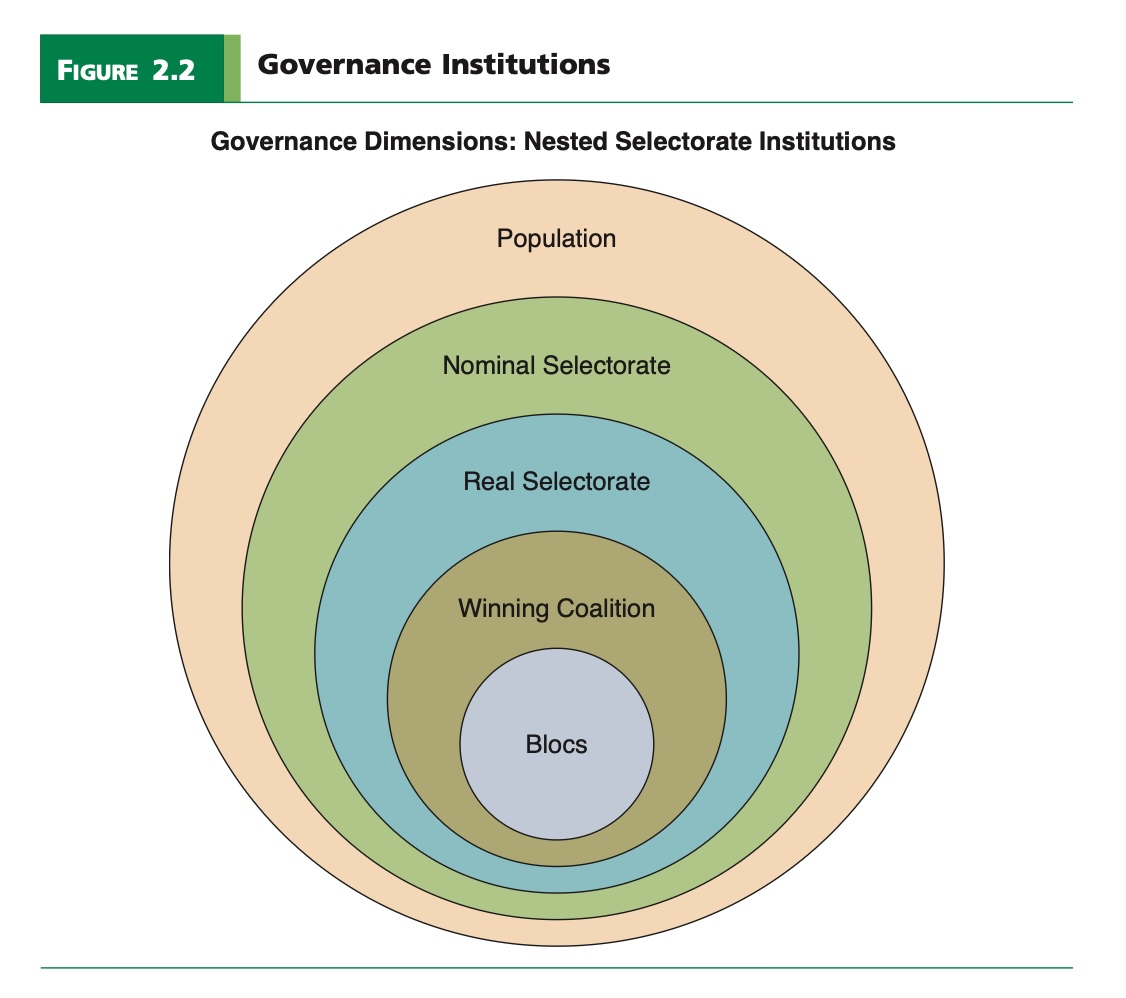
\includegraphics[width=0.7\textwidth]{images/nested_selectorate_institutions.jpg}
    \captionof{figure}{\label{fig:fig3_nested_selectorate_institutions}%\textit{\parencite[Fig.\(\backsim\)1]{cranmerWhatCanWe2017}}
    }
\end{center}

When domestic institutions constrain a leader to require a broad base of support private rewards are an inefficient way to retain power (de Tocqueville 2000; Lake and Baum 2001; Bueno de Mesquita et al. 2003; Bueno de Mesquita and Smith 2011). Democratic leaders would have to spread these rewards across so many people that each would receive too little for the benefits to influence their loyalty to the incumbent.

When political institutions compel a leader to depend on many supporters so that a bundle of public goods is the reward for retaining the incumbent, \textbf{the institutions of governance induce weak loyalty to the incumbent}.



\newpage
\part{Session 4}
\textbf{Session 4, March 2: Bargaining theory of war}

\begin{itemize}
    \item [***] \textcite{lakeTwoCheersBargaining2010}
    \item \textcite{Fearon_1995}
    \item \textcite{sechserCrisisBargainingNuclear2013}
    \item \textcite{powellInefficientUsePower2004}
\end{itemize}
% Session 04 summaries: designed to be included from an existing main.tex
% No documentclass, packages, or document environment are included.

\section{James D. Fearon -- Rationalist Explanations for War}

\subsection{Central Puzzle and the Bargaining Framework}

The article asks how war can arise between genuinely rational, unitary states whose leaders understand the costs of fighting. Fearon distinguishes this question from explanations based on irrationality or domestic political pathologies. His goal is narrower and foundational.

The key move is to treat war as a bargaining problem. Suppose two states dispute an issue that can be divided along a continuous interval. If state A wins a war with probability p and both states pay positive costs of fighting, then war is a costly lottery. A's expected payoff from war is p minus its costs, while B's is 1-p minus its costs. Because both sides lose something by fighting, there normally exists a set of peaceful divisions that gives each side more than its expected payoff from war. This set is the bargaining range. In the risk-neutral case, the width of the range is essentially the sum of the two sides' costs of war. Risk aversion makes the peaceful range even larger.

This result shifts the explanatory burden. It is not enough to say that a leader expects the benefits of war to exceed the costs. Even if war has positive expected utility, both sides should still prefer a bargain that reproduces the expected distributional outcome without paying the costs of combat. War is ex post inefficient, and this inefficiency normally creates an ex ante space for agreement. A coherent rationalist theory of war must therefore explain why states cannot locate or agree on a settlement inside that range.

\begin{center}
    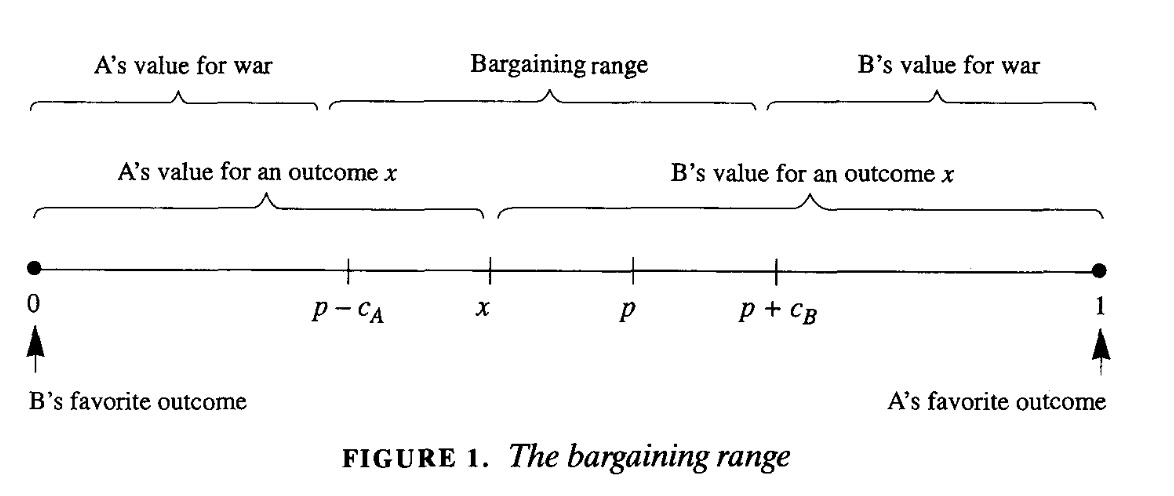
\includegraphics[width=1\textwidth]{images/fearon_rationalist_explanations_war_bargaining_range.jpg}
    \captionof{figure}{\label{fig:fig7_fearon_rationalist_explanations_war_bargaining_range.jpg}%\textit{\parencite[Fig.\(\backsim\)1]{cranmerWhatCanWe2017}}
    }
\end{center}

\subsection{Why Standard Rationalist Arguments Are Incomplete}

Fearon evaluates several familiar explanations.

The central question, then, is what prevents states in a dispute from reaching an ex ante agreement that avoids the costs they know will be paid ex post if they go to war?

\begin{enumerate}
    \item First, \textbf{anarchy} by itself is insufficient. The absence of a world government may permit the use of force, but \textbf{it does not explain why states choose an option that destroys resources when mutually preferable bargains are available}.
    
    \item The \textbf{security dilemma} similarly can generate fear, arms races, and competition, but unless one specifies how the absence of enforceable commitments blocks a peaceful bargain, the argument does not solve the bargaining puzzle.
    
    Security dilemma: the fact that under anarchy one state's efforts to make itself more secure can have the undesired but unavoidable effect of making another state less secure.

    \item Second, the standard \textbf{preventive-war} argument is incomplete. A declining state may fear that a rising state will become stronger and exploit it later. But this immediately raises a bargaining question: why cannot the rising state make concessions today and promise future concessions sufficient to induce the declining state not to attack? The problem is not power shifts in themselves. Preventive war becomes a genuine rationalist explanation \textbf{only when} the changing balance of power creates a \textbf{commitment problem}--when the rising state cannot credibly commit not to use its future strength to revise the agreement.
    \item Third, positive \textbf{expected utility} for war is not enough. Two states can both believe that war is worthwhile relative to the status quo and \textbf{still possess a bargaining range that would make both better off}.
    \item Finally, \textbf{issue indivisibility} is logically capable of eliminating the bargaining range, but Fearon treats it as empirically less compelling. Most international disputes are multidimensional, and side payments, issue linkages, partitions, alternation, or lotteries can often create intermediate outcomes. When issues appear indivisible in practice, the deeper cause may be nationalism, domestic political constraints, or some other mechanism rather than a natural indivisibility of the issue itself.
\end{enumerate}

\subsection{Private Information and Incentives to Misrepresent}
Fearon's first major mechanism combines private information with strategic incentives to misrepresent it. Leaders may possess information about military capabilities, tactics, resolve, or the value they attach to the disputed issue that the opponent does not know. This can create divergent estimates of the likely outcome of war or of the opponent's willingness to fight. Yet simple uncertainty is not sufficient: \textbf{because war is costly, rational states have incentives to reveal information to avoid an inefficient conflict}.

The problem is that bargaining creates incentives to bluff. This logic explains why rational miscalculation can persist.

States can in principle communicate with each other and so avoid a costly miscalculation of relative power or will. The cause of war cannot be simply lack of information, but whatever it is that prevents its disclosure. I argue that the fact that states have incentives to misrepresent their positions is crucial here, explaining on rationalist terms why diplomacy may not allow rational states to clarify disagreements about relative power or to avoid the miscalculation of resolve.

The same reasoning applies to disputes about relative power. Conflicting expectations can shrink or eliminate the apparent bargaining range, but rational actors must have some basis for holding different beliefs. Private information about capabilities is one source. Yet the critical mechanism is again the difficulty of credibly revealing that information. The article therefore recasts many traditional claims about miscalculation as specific bargaining failures produced by asymmetric information and incentives to dissemble.

\section{James D. Fearon -- Rationalist Explanations for War}
\subsection{The central puzzle and Fearon's objective}
Fearon begins from a simple but fundamental puzzle: wars are costly, risky, and destructive, yet they repeatedly occur. Existing explanations can be divided into three broad families. One attributes war to irrationality, psychological biases, or pathologies among leaders. A second focuses on domestic political distortions, in which leaders may enjoy the benefits of war while shifting much of its cost onto soldiers and citizens. Fearon concentrates on a third possibility: whether war can occur even when states are treated as rational, unitary actors whose leaders take the costs and risks of fighting seriously.

This question matters not only for the study of war but also for neorealist international relations theory. If war cannot be explained among rational unitary states, then the roots of conflict must lie primarily in individual or domestic-level defects rather than in the international system itself. Fearon's aim is therefore to identify the set of rationalist explanations that are both logically coherent and empirically plausible.

His central criticism of much of the existing literature is that it asks the wrong question. It is not enough to show that war might have a positive expected value, that states live under anarchy, that one state is declining, or that leaders can miscalculate. Because fighting is costly, rational states should normally have an incentive to search for a negotiated settlement that gives both sides more than they expect to obtain from war after subtracting the costs of fighting. A satisfactory rationalist theory must therefore explain why such a bargain cannot be located or credibly implemented before the war begins.

% (1) anarchy; (2)
% expected benefits greater than expected costs; (3) rational preventive war; (4)
% rational miscalculation due to lack of information; and (5) rational miscalcula-
% tion or disagreement about relative power. I argue that the first three
% arguments simply do not address the question of what prevents state leaders
% from bargaining to a settlement that would avoid the costs of fighting. The
% fourth and fifth arguments do address the question, holding that rational
% leaders may miss a superior negotiated settlement when lack of information
% leads them to miscalculate relative power or resolve. However, as typically
% stated, neither argument explains what prevents rational leaders from using
% diplomacy or other forms of communication to avoid such costly miscalcula-
% tions.

Fearon reviews five familiar rationalist arguments:
\begin{enumerate}
    \item anarchy
    \item positive expected utility from war
    \item preventive war
    \item miscalculation caused by incomplete information
    \item disagreement about relative power
\end{enumerate}

Fearon argues that the first three do not directly solve the bargaining puzzle. The last two move closer to a solution but are incomplete unless one explains why diplomacy cannot reveal the relevant information.

The article ultimately identifies two major mechanisms capable of explaining rational war: \textbf{private information combined with incentives to misrepresent it}, and \textbf{commitment problems}.

A third possibility, \textbf{issue indivisibility}, is logically possible but is treated as less compelling empirically.

\subsection{War as a bargaining failure}
The key theoretical move is to treat war as an inefficient bargaining outcome rather than simply as another policy option. Fearon distinguishes between \textit{ex ante} and \textit{ex post} efficiency. A war can be attractive to a state before fighting if the expected gains exceed the expected costs. Yet war remains inefficient ex post as long as the parties incur positive costs in obtaining an outcome that, in principle, could have been allocated through negotiation without paying those costs. Even a ``wanted'' war therefore poses a rationalist puzzle.

Suppose two states, A and B, bargain over an issue represented by the interval $[0,1]$. State A prefers outcomes closer to 1, while B prefers outcomes closer to 0. If war occurs, A wins with probability $p$ and B with probability $1-p$. Let $c_A$ and $c_B$ denote the costs of war to A and B. In the simplest risk-neutral formulation, A's expected payoff from war is

\[
p-c_A,
\]

while B's expected payoff is

\[
1-p-c_B.
\]

A peaceful settlement $x$ is preferable to war for A when

\[
x>p-c_A,
\]

and preferable for B when

\[
1-x>1-p-c_B,
\]

which is equivalent to

\[
x<p+c_B.
\]

Therefore every agreement in the interval

\[
(p-c_A,\;p+c_B)
\]

is preferred by both states to war. This interval is the \textbf{bargaining range}. Its width is $c_A+c_B$: the costs of war create a wedge within which mutually beneficial settlements exist.

Fearon's intuitive example is a dispute over a division of 100 dollars. If each side has a 50 percent chance of winning all 100 dollars in war but must pay a cost of 20 dollars to fight, each has an expected war payoff of 30 dollars. Any negotiated split giving each side more than 30 dollars is therefore better than war. The exact distribution of gains can be contentious, but the existence of a bargaining range means that disagreement over distribution alone cannot explain why rational actors pay the additional costs of war.

This result depends on several assumptions, but Fearon argues that they are relatively weak. The states must recognize that there is some true probability of victory, they must be risk-neutral or risk-averse rather than strongly risk-loving, and the issue must allow a sufficiently continuous range of settlements. \textbf{Risk aversion actually enlarges the set of bargains preferable to war, because a certain compromise is more attractive relative to a risky all-or-nothing contest.}

The implication is crucial: the fact that a leader believes war has positive expected utility does not by itself explain war. Even if both states prefer fighting to the status quo, there may still be negotiated settlements that both prefer to fighting. The appropriate question is therefore not ``Why might war be attractive?'' but \textbf{``Why do states fail to reach an agreement inside the bargaining range?''}

\subsection{Why standard explanations are insufficient}

\subsubsection{Anarchy}
Under anarchy, no sovereign can automatically punish states for using force, and each state must provide for its own security. Fearon accepts that this condition is fundamental to international politics, but he argues that the usual formulation is incomplete. Saying that \textbf{nothing prevents states from fighting does not explain why they choose a costly option when mutually preferable bargains should be available.}

The same criticism applies to standard versions of the \textbf{security dilemma}. One state's defensive measures may threaten another, encouraging arms races and spirals of fear, but this still does not explain why rational states cannot bargain around the danger. To turn anarchy into a true rationalist explanation, one must identify a specific mechanism through which the absence of enforcement makes a mutually preferred bargain impossible to sustain.

Fearon later provides such a mechanism through commitment problems.

\subsubsection{Preventive war}

A common argument holds that a declining state may rationally attack a rising state before the balance of power shifts further against it. Fearon notes that this reasoning also skips the bargaining question. If the rising power wants to avoid being attacked while it is still relatively weak, why can it not compensate the declining power with present or future concessions? \textbf{The important issue is not the power shift itself but} whether the rising state can \textbf{credibly commit} to respect a bargain after it becomes stronger. \textbf{Preventive war is therefore best understood as a commitment problem}, not simply as a consequence of changing relative power.

\subsubsection{Positive expected utility}

The claim that leaders fight whenever the expected benefits of war exceed the expected costs similarly fails. Positive expected utility can make war preferable to the status quo, but it does not show that war is preferable to every possible negotiated settlement. As long as the issues are sufficiently divisible and war is costly, the bargaining range persists.

\subsection{Issue indivisibility}

Issue indivisibility is the third logically coherent route to rational war identified by Fearon, but he regards it as empirically weaker than the two main mechanisms. If an issue can take only a small number of discrete outcomes, it is possible that none lies inside the bargaining range. A dispute over which prince occupies a throne, for example, may appear inherently all-or-nothing.

Fearon nevertheless stresses that most international disputes are multidimensional. States can often use side payments, link several issues together, divide territory, alternate control, or devise probabilistic arrangements. Historically, rulers bought and sold territory, and even seemingly indivisible issues can sometimes be transformed into divisible bargains. \textbf{If intermediate agreements are politically impossible, the deeper explanation may lie in nationalism, domestic institutions, legitimacy, or other mechanisms rather than in the physical nature of the issue itself}. Thus issue indivisibility can explain war in principle, but one should first ask why the parties cannot construct a divisible settlement.

\subsection{Private information and incentives to misrepresent}

The first major mechanism begins with incomplete information. Leaders may possess private information about their military capabilities, war plans, the reliability of allies, their willingness to endure costs, or the value they attach to the disputed issue. This can lead states to disagree about the probable outcome of war or to misjudge an opponent's resolve.

\textbf{Private information alone is not enough. If both states genuinely want to avoid the costs of war, they should have incentives to reveal information} that would prevent a disastrous miscalculation. The real question is why such information cannot be credibly communicated.

Fearon's answer is that bargaining also creates incentives to \textbf{misrepresent}. A state that appears stronger or more resolved can obtain a better deal, so weak or low-resolve states may bluff. Conversely, states may hide genuine capabilities or plans because revealing them would sacrifice military advantages. As a result, messages are strategically distorted and cannot automatically resolve uncertainty.

\subsubsection{Disagreement about relative power}

A well-known argument, associated with Geoffrey Blainey, holds that wars often begin when states disagree about their relative strength. If both sides are optimistic about victory, their reservation values may overlap so little that the perceived bargaining range disappears. Yet Fearon asks how two fully rational actors can sustain incompatible estimates of the same military contest.

Under a strict rationalist interpretation, conflicting estimates must arise from different information. If two rational actors possessed the same information, they should reason toward the same probability assessment. Differences produced merely by cognitive limitations, nationalist enthusiasm, or inability to process complex evidence are better understood as bounded-rationality explanations rather than pure rationalist ones.

States clearly do possess private military information. The problem is that, in principle, they could share it. Therefore the causal chain must include an explanation for why credible disclosure fails. Incentives to hide capabilities, exaggerate strength, preserve surprise, or avoid exposing strategy provide that missing link.

The Russo-Japanese War of 1904 illustrates the argument. Russian leaders were highly confident that Russia would defeat Japan and therefore resisted Japanese proposals concerning Korea and Manchuria. Japanese leaders were much less pessimistic about their own prospects because they possessed better information about Japanese military reforms, intelligence, and Russian weaknesses in Northeast Asia. Japan could not simply announce that its forces were stronger than Russia believed: Moscow would have had little reason to trust the claim. Nor could Japan reveal the operational information supporting its confidence without undermining the military advantage itself. The bargaining failure thus reflected both private information and the strategic difficulty of credibly revealing it.

\subsubsection{Miscalculation of resolve}

A related explanation concerns uncertainty about willingness to fight. State A may challenge an interest of state B because it mistakenly believes B will not resist. Fearon lists familiar examples: German uncertainty about Russian and British resolve in 1914, Hitler's expectations concerning Britain and France, Japanese assessments of U.S. willingness to fight in 1941, North Korea's expectations about American intervention in 1950, and U.S. uncertainty about Chinese intervention in Korea.

A simple bargaining model clarifies the logic. A challenger chooses how much of the status quo to revise, while the target can accept the revision or fight. Under complete information, the challenger will normally demand just enough to leave the target indifferent between acceptance and war, avoiding conflict. Under incomplete information about the target's costs or resolve, however, the challenger faces a trade-off: a larger demand yields greater gains if accepted but also increases the probability that the target will fight. If the challenger's own costs of war are not too high, its optimal strategy may rationally involve a positive probability of war.

This shows that war does not require disagreement about relative power. Even if both sides agree about military capabilities, uncertainty about how much the opponent values the issue can be sufficient. But again, the explanation is incomplete unless one explains why the target cannot simply communicate its resolve.

\subsubsection{Cheap talk and costly signaling}

\textbf{If statements are costless, the problem is severe.} This is the logic of \textit{cheap talk}: when all actors would like to send the same intimidating message regardless of their true type, the message carries little information.

Signals become more informative when they are costly in ways that low-resolve states are less willing to bear. Many credible signals are costly precisely because they intail the risk of escalation.

Mobilizing forces, building weapons, signing alliances, stationing troops abroad, risking international reputation, or creating domestic political audience costs can make threats more credible. 

The July 1914 crisis illustrates these dynamics. German leaders received warnings that Russia might fight if Austria-Hungary moved against Serbia, but they discounted verbal statements because Russia had an obvious incentive to bluff. At the same time, German leaders had incentives to conceal the extent of their support for Austria-Hungary, partly because open disclosure would make Germany appear responsible for escalation and could affect domestic and British opinion. Misrepresentation on both sides made clear communication difficult. As mobilizations and other costly signals accumulated, backing down became harder and the risk of war rose.

Fearon also emphasizes \textbf{reputational mechanisms}. A state may fight today because conceding would reveal that its costs of fighting are high, inviting future challenges. War itself can then serve as a costly signal of resolve. Similarly, a rising power may use conflict to demonstrate capabilities that others underestimate. These mechanisms are not irrational: they arise because information valuable in bargaining is private and because actors have strategic reasons to conceal or distort it.

\subsection{Commitment problems}

The second major mechanism can produce war even under complete information. The parties may know each other's capabilities, preferences, and intentions and still fail to reach peace because they cannot \textbf{credibly commit to uphold an agreement}. \textbf{Here anarchy matters in a precise way: no external authority can enforce promises when one side later acquires an incentive to defect.}

Fearon discusses three forms of commitment problem: preemptive war caused by first-strike advantages, preventive war caused by shifts in relative power, and bargaining over strategically important territory that changes future bargaining power.

\subsubsection{Preemptive war and first-strike advantages}

Fearon uses the analogy of two gunslingers. Both prefer mutual peace to a gunfight, but each would most prefer to kill the other by surprise. If neither can commit not to exploit an opportunity for a first strike, peaceful coexistence may be unstable even though both would prefer it to mutual fighting.

In international politics, this logic can arise when military technology or geography provides a large advantage to attacking first. Let $p_f$ be A's probability of victory if it strikes first and $p_s$ its probability if it strikes second. A strong first-strike advantage means $p_f>p_s$. Peaceful agreements are self-enforcing only if both states prefer to respect them rather than defect by attacking. In the risk-neutral case, the effective bargaining range exists only when:
\[ p_f-c_A < p_s+c_B.\]
If the first-strike advantage becomes sufficiently large relative to the costs of war, the interval of self-enforcing bargains can disappear. Importantly, mutually preferable agreements may still exist abstractly; the problem is that neither state can credibly promise not to exploit the advantage of attacking first.

Fearon is cautious about the empirical importance of the pure preemption mechanism. Even in 1914, when leaders often believed that striking first conferred significant advantages, they did not generally behave as if war were inevitable regardless of diplomacy. First-strike advantages may therefore be more important as an aggravating factor: they narrow the set of enforceable bargains and make informational problems and costly signaling more dangerous.

\subsubsection{Preventive war as a commitment problem}

Preventive war is more empirically significant. Suppose A is rising and will be more powerful tomorrow, while B is declining. Even if A promises today not to exploit its future strength, that promise may be incredible because once the power shift occurs A will have an incentive to demand more. B therefore evaluates not only the present status quo but also the less favorable bargain it expects to face in the future.

This reframes preventive war. The declining state does not necessarily attack because it expects the rising state to invade later. It may attack because it expects future peace to occur on much worse terms. War today can be rational if the future shift in bargaining power is sufficiently large relative to the costs of fighting and if the rising state cannot credibly limit its future demands.

The logic helps explain why simple power-transition arguments are incomplete. \textbf{Power shifts cause war only when they generate a commitment problem.} If the rising state can credibly transfer resources, limit its future power, or otherwise compensate the declining state, war may be avoided. Fearon notes that the historical practice of compensation in classical balance-of-power politics can be interpreted as an attempt to reduce preventive incentives.

The origins of World War I contain this logic. German and Austro-Hungarian leaders worried about the rapid growth of Russian power. Their concern was not only that Russia might eventually attack, but that a stronger Russia would possess greater bargaining leverage in the Balkans and the Near East, potentially threatening the internal stability of Austria-Hungary. Russia could not credibly promise that, once stronger, it would refrain from using this leverage. Preventive motives therefore made German leaders more willing to accept the risks of escalation in 1914, even if Fearon does not claim that this mechanism alone caused the war.

\subsubsection{Strategic territory and appeasement}
A similar commitment problem arises when the object being negotiated is itself a source of military or economic power. Territory may contain resources, defensible positions, transportation routes, or strategic depth. A small concession can therefore change the future distribution of power and alter subsequent bargaining.

Suppose one state is willing to make a limited territorial concession to avoid war. If receiving the territory would make the other state much stronger, however, the recipient may later use its new advantage to demand still more. The recipient cannot credibly commit not to exploit the shift, so the weaker state may rationally reject even a limited concession and choose war instead. What appears to be issue indivisibility may actually be a commitment problem.

Fearon illustrates this with the 1939 Winter War. Stalin sought territorial adjustments and islands near Leningrad that the Soviet Union regarded as strategically important. Finnish leaders feared that making these concessions would improve the Soviet position and allow Moscow to press for additional gains later, especially given Soviet behavior in the Baltic states. If Stalin could not credibly commit to stop after the initial concessions, Finland could rationally reject an agreement that both sides might otherwise have preferred to war. The resulting conflict therefore demonstrates how strategic territory can make appeasement difficult even when neither side positively desires a costly war.

\subsection{Conclusion and implications}

Fearon's article advances two principal conclusions. First, because war is costly and risky, negotiated settlements that both sides prefer to fighting should exist under broad conditions. Rationalist theories cannot simply assume a deadlock in which war is the only mutually acceptable option. The existence of a bargaining range is the starting point for analysis.

Second, the most coherent rationalist explanations for war identify mechanisms that prevent states from locating or implementing agreements in that range. The two central mechanisms are \textbf{information problems}---private information about capabilities or resolve combined with incentives to misrepresent---and \textbf{commitment problems}---situations in which one or both states cannot credibly promise to respect an agreement in the future. Issue indivisibility is possible but is often better understood as the consequence of deeper political or commitment mechanisms.

These mechanisms do not imply that irrationality or domestic politics are unimportant. Fearon explicitly argues the opposite: \textbf{clarifying what rational unitary actors should be able to achieve makes it easier to identify where bounded rationality, nationalism, regime incentives, or other domestic factors are doing explanatory work.}

For example, if disagreements about military strength were driven mainly by rational private information, leaders should update their beliefs about an opponent's capabilities when that opponent takes unexpectedly tough bargaining positions. Fearon notes that historical evidence of such updating about capabilities is difficult to find, even though updating about resolve appears much more common. This observation leaves substantial room for bounded rationality in empirical explanations of war.

A second limitation is that anarchy and private information are pervasive features of international politics, while war is relatively rare. Fearon accepts this point. The two mechanisms are not by themselves predictions that war must occur; rather, they are foundational causal logics. Specific models must identify the variables that activate them in particular settings---for example, the size and speed of a power shift, the costs of war, the size of a first-strike advantage, the strategic value of territory, or the distribution of private information.

The broader theoretical implication is a demanding standard for explanations of war. A proposed cause such as multipolarity, offensive advantage, failure to balance, or changing relative power is not yet a complete rationalist explanation. To show how it causes war among rational unitary states, one must demonstrate how it generates either an information problem that cannot be resolved without risk or a commitment problem that makes peaceful bargains unenforceable. In this sense, Fearon's bargaining framework reorganizes a large and fragmented literature around a common question: if peace would save both sides the costs of fighting, what specific strategic obstacle prevents them from reaching it?

\clearpage

\section{Robert Powell -- The Inefficient Use of Power: Costly Conflict with Complete Information}

\subsection{The Inefficiency Puzzle}

Powell studies a broad political puzzle: actors sometimes use costly forms of power even though they could, in principle, reach an agreement that leaves everyone better off. Examples include war, civil war, coups, revolutions, policy insulation, and other forms of coercion. The use of power consumes resources, so the total benefits available before conflict are larger than those remaining afterward. The central question is therefore why bargainers sometimes fail to reach a Pareto-superior settlement before power is used.

\begin{enumerate}
    \item \textbf{Powell concentrates on commitment problems that can produce bargaining breakdown even under complete information.}
    \item The actors may know each other's preferences, capabilities, and options perfectly, yet still be unable to sustain an efficient agreement because future incentives make promises incredible.
\end{enumerate}

\subsection{A Common Commitment Problem Across Political Settings}

The common structure is dynamic. Actors bargain over a flow of benefits rather than a single one-time pie. They cannot fully commit today to how future benefits will be divided, and the amount each actor can guarantee itself through the use of power changes over time. When the strategic environment shifts rapidly, an agreement that is attractive today may cease to be incentive-compatible tomorrow. This makes efficient bargaining dynamically inconsistent.

Powell illustrates the mechanism through several existing models. In Acemoglu and Robinson's work on political transitions, rich and poor factions compete for control. A temporarily powerful faction may be bought off only if transfers continue for several periods. Yet when political or economic conditions change, the faction promising future concessions gains an incentive to renege. Anticipating this, the temporarily strong faction may prefer a costly coup or revolution now.

Fearon's model of secessionist civil war has a similar logic. When the government is temporarily weak, rebels have a window of opportunity. The government would like to offer enough regional control to induce peace, but the rebels' value of fighting may exceed what can be transferred in a single period. A sufficient concession therefore requires a multi-period promise. If the government is likely to become strong again, however, it will later prefer to retract the concessions. Knowing this, the rebels fight while the opportunity exists, even though both sides would prefer an enforceable peaceful arrangement.

De Figueiredo's model of policy insulation provides a domestic analogue. A politically weak party that happens to be in office may deliberately make its policy difficult and costly to reverse. Such insulation is inefficient, but the party expects to lose power and cannot trust its opponent to preserve the policy later. The ability of the future majority to overturn today's policy makes reciprocal restraint difficult to sustain.

Powell's own preventive-war model shows the same pattern in international politics. A declining state bargains with a rising state whose probability of military victory increases over time. The rising state would prefer to promise the declining state a favorable territorial settlement in order to avoid war. Yet as the rising state grows stronger, its payoff from fighting increases and it becomes less willing to respect the earlier bargain. If the change in power is sufficiently large and rapid, the declining state rationally prefers to fight before its position worsens.

\subsection{The General Mechanism: Shifts in Bargaining Power}

Across these cases, a temporarily weak actor needs to buy off an adversary that currently possesses a valuable option to use power. Because the use of power is costly, there are enough total resources to make peaceful accommodation desirable. The difficulty is that resource constraints often prevent the needed compensation from being paid immediately. The transfer must instead be spread across a concession phase lasting several periods.

During this concession phase, the strategic environment may change. The actor that is weak today may become strong tomorrow. Once stronger, it can secure a better outcome by abandoning the promised transfers. Since the future beneficiary anticipates this, the promise is not credible today. Thus the problem is not ignorance about future power: all changes can be common knowledge. Nor is it simply impatience. The breakdown comes from the interaction of limited current transfers, inability to commit to future transfers, and a sufficiently rapid shift in the distribution of bargaining power.

This is why complete information does not guarantee efficiency. In a static bargain, knowing all payoffs would normally allow the actors to divide the surplus. In a changing environment, however, the allocation that would induce restraint today may require behavior tomorrow that will no longer be optimal for the actor making the promise. The use of power becomes a way to lock in an outcome before the strategic balance changes.

\subsection{The Inefficiency Condition}

Powell formalizes the argument in a two-player stochastic game. A stochastic game differs from a standard repeated game because the strategic environment can move among different states. Each actor has a minmax payoff in every continuation game: the minimum payoff it can guarantee itself regardless of what the opponent does. Powell treats these minmax payoffs as a measure of relative bargaining power because they capture what an actor can lock in through its own actions.

The core inefficiency condition states, in substance, that an efficient path cannot be sustained when at some point an actor can guarantee itself more by deviating than it can receive while continuing to cooperate. One useful interpretation is a 'lock-in' condition: if one actor's current guaranteed payoff plus the discounted amount the other actor can guarantee itself in the next period exceeds the total flow of benefits available, both claims cannot simultaneously be satisfied. There is then no efficient equilibrium at that point.

A second and especially intuitive interpretation compares the expected shift in an actor's minmax payoff with the bargaining surplus. If the expected increase in one side's guaranteed future payoff is larger than the surplus generated by avoiding costly conflict, no feasible sequence of transfers can keep both sides satisfied. In less formal terms, large and rapid changes in relative power can make all equilibria inefficient. The speed and magnitude of the change matter because they determine how quickly today's credible concessions become tomorrow's unattractive promises.

A third interpretation emphasizes the limit on credible transfers. An actor can compensate its opponent partly in the current period and partly through promised future transfers. Yet future promises are bounded by what the promisor will voluntarily honor once the strategic environment changes. If the opponent's current minmax payoff exceeds the sum of what can be transferred now and what can credibly be promised later, the use of power cannot be bought off.

\subsection{Stable Environments and the Broader Contribution}

Powell contrasts stochastic games with infinitely repeated games. In an ordinary repeated game the strategic environment does not change: the same stage game recurs indefinitely. Because continuation values remain stable, there are no large jumps in minmax payoffs to undermine future cooperation. If actors are sufficiently patient, standard folk-theorem results therefore allow efficient equilibria. This comparison underscores that the source of inefficiency in Powell's argument is not repetition itself but rapid movement in the distribution of bargaining power.

The broader contribution is to unify diverse literatures. Coups, revolutions, civil wars, preventive wars, and policy insulation can all be understood as manifestations of the same commitment problem. A temporarily favorable opportunity to use power becomes attractive when an opponent cannot credibly promise the concessions required to make restraint worthwhile over time. The article therefore generalizes the bargaining logic of commitment problems beyond international war.

Powell also identifies an agenda for future research. His general model treats shifts in power largely as exogenous: governments become strong or weak, parties gain or lose office, and military balances change. Explaining the microfoundations of those shifts--why they occur, how quickly they occur, and when political actors can influence them--is essential for determining where the inefficiency mechanism should be most important empirically. The main theoretical lesson nevertheless remains clear: costly conflict does not require hidden information. Even with complete information, rapid changes in relative power combined with limited commitment can make efficient bargaining impossible.

\clearpage

\section{Sechser \& Fuhrmann -- Crisis Bargaining and Nuclear Blackmail}

\subsection{Research Question and Main Argument}

Sechser and Fuhrmann ask whether nuclear weapons give states an advantage when they try to compel other states to make concessions.

\begin{enumerate}
    \item \textbf{Deterrence:} seeks to prevent an opponent from changing the status quo.
    \item \textbf{Compellence:} seeks to make an opponent take an action, reverse a policy, or relinquish something it already possesses.
\end{enumerate}

A common view holds that nuclear weapons cast a \textbf{Devo ritornare su questo punto $\Rightarrow$ 'looming shadow'} over crisis bargaining. Because nuclear states can inflict extraordinary destruction, targets should be more willing to comply with their demands. The supposed advantage may be greatest when only the challenger has nuclear weapons, because the target cannot retaliate in kind. Some scholars further claim that the effect does not require an explicit nuclear threat: simple possession of a nuclear arsenal may increase the challenger's leverage.

The authors reject this logic. Their central claim is that nuclear weapons are uniquely poor instruments of compellence. Successful compellent threats are especially plausible when a challenger can
\begin{itemize}
    \item credibly threaten to seize the disputed object by force
    \item when carrying out the threatened punishment would impose relatively low costs on the challenger
\end{itemize}
Nuclear weapons satisfy neither condition.

\subsection{Why Nuclear Weapons Are Weak Compellent Tools}

\begin{enumerate}
    \item \textbf{Nuclear weapons are not useful tools of conquest.} Many compellent disputes concern territory, cities, or other objects that the challenger wants to acquire. Conventional military forces can threaten to take and hold such objects, which may induce a target to concede rather than fight a losing war. Nuclear weapons, by contrast, are designed for destruction.
    \item \textbf{Punishment:} Instead, a nuclear state might hope to coerce a target by threatening to attack the target's valued possessions. A challenger could threaten to incinerate a target state's capital city, for example, unless it relinquished a disputed territory. But this possibility highlights a second limitation of nuclear weapons: \textbf{the costs of executing nuclear punishment likely would be tremendous}. Tha state would provoke an international backlash, potentially triggering economic sanctions and international isolation, encouraging nuclear proliferation, and provoking other states to align against it. Indeed, \textbf{the fact that the challenger has already lived without the item for some period of time suggests that it could continue to do so, even if it would rather not.}
\end{enumerate}

Deterrence and compellence should have different nuclear dynamics: When a state's \textbf{survival} is directly threatened, \textbf{the enormous costs of nuclear use may still be acceptable}, making a deterrent threat credible. Compellent demands usually involve objectives that are valuable but not vital.

\subsection{Problems in Earlier Research}

The article argues that previous studies often cannot answer the comparative question properly. Many qualitative studies select only famous nuclear crises, especially Cold War episodes involving the United States. Such designs lack a nonnuclear comparison group, so they cannot establish whether nuclear states are more successful than comparable nonnuclear states. Selecting famous or prolonged crises may also overrepresent failed coercive threats, because successful threats often end crises quickly and quietly.

Existing quantitative datasets create a different problem. Datasets such as International Crisis Behavior and Militarized Interstate Disputes contain many episodes in which no compellent threat was made at all. They also often classify battlefield victories as crisis successes. This confuses brute-force achievement with coercive success. For the authors, a successful threat is one that obtains compliance without the challenger having to carry out major military force. The 1991 Gulf War illustrates the distinction: the coalition won militarily, but the prewar ultimatum compelling Iraq to leave Kuwait failed because Iraq refused and war followed.

\subsection{Research Design and Measurement}

The dataset contains interstate compellent threats from. The dataset includes nuclear and nonnuclear challengers, famous and obscure crises, and cases in which nuclear weapons were or were not discussed.

The dependent variable, compellence success, equals one only when the target voluntarily complies with all of the challenger's demands and the challenger does not need to use military force to obtain the outcome. Roughly 30 percent of the threats in the dataset meet this standard. The main explanatory variables measure whether the challenger possesses nuclear weapons, whether the target is nuclear armed, and the interaction between the two. The authors also test alternative measures such as arsenal size, nuclear superiority, the nuclear capability ratio, and the numerical difference in arsenal size.

The statistical models control for important alternative explanations.
\begin{itemize}
    \item Conventional capability matters because a state with superior nonnuclear military power may be more coercively effective regardless of its nuclear arsenal.
    \item The stakes variable distinguishes demands over territory or leadership from lower-stakes disputes.
    \item Probit models estimate the probability that a compellent threat succeeds, with clustered standard errors to account for repeated observations of some country pairs.
\end{itemize}

\subsection{Empirical Findings}
\begin{itemize}
    \item \textbf{The results provide no support for the claim that nuclear weapons improve compellent bargaining performance.}
    \item nuclear states do not gain a reliable advantage even when the target lacks nuclear weapons.
    \item The conclusion remains unchanged when nuclear power is measured in different ways.
    \item Larger arsenals, nuclear superiority over the target, nuclear capability ratios, and absolute differences in arsenal size do not provide robust evidence of a compellent advantage.
\end{itemize}

The central empirical result is therefore not simply that explicit nuclear threats rarely occur, but that possession itself does not appear to cast the coercive shadow claimed by the nuclear-blackmail argument.

\subsection{Limitations, Implications, and Conclusion}
\begin{itemize}
    \item This study demonstrates that nuclear weapons do not have the coercive leverage that their extraordinary power might sugges.
    \item Weapons that are exceptionally powerful may be politically unusable when carrying out the threat would impose enormous costs on the coercer or fail to deliver the object being demanded.
    \item The study cannot evaluate whether \textbf{explicit} nuclear compellent threats would work better, because leaders have almost never made clear, unambiguous threats to use nuclear weapons in support of compellent demands.
    \item The analysis focuses on peacetime threats and therefore leaves \textbf{open whether nuclear weapons might have greater compellent value once a war has already begun}.
    \item The theoretical implication is broader than nuclear politics:
    \[destructive\ capability\ \not =\ coercive\ leverage\]
    \item The \textbf{practical implication} concerns proliferation fears. \textbf{Policymakers} often warn that new nuclear states would be able to blackmail weaker neighbors. The historical record examined here provides little support for that fear.
\end{itemize}


\newpage
\part{Session 5}
\textbf{Session 5, March 9: Domestic theories of war}
\begin{itemize}
    \item [***] \textcite{buenodemesquitaPrinciplesInternationalPolitics2013}{ Chapter 6}
    \item \textcite{allisonConceptualModelsCuban1969}
    \item \textcite{buenodemesquitaDomesticExplanationsInternational2012}
    \item \textcite{putnamDiplomacyDomesticPolitics1988}
    \item \textcite{bendorRethinkingAllisonsModels1992}
\end{itemize}

\section{Bueno de Mesquita, 2013 Chapter 6, Domestic Theories of War}

\begin{enumerate}
    \item War is correctly viewed as ex post inefficient from the perspective of national welfare; however, it can be efficient for leaders, especially those who head a small-coalition, autocratic government.

    \item When domestic politics plays a part in shaping demands for war, it can increase the credibility of threats, reduce the likelihood of threats, and alter the path of conflict escalation.

    \item Domestic politics alter the subject matter of war. Domestic accountability makes the pursuit of policy concessions and regime change focal issues for democracies. In autocracies, the focal issues for which wars are fought involve resource acquisition and territorial conquest.

    \item Democrats try harder to win the wars they fight than do autocracies, and democracies are more selective about their preparedness to fight. Selection effects identified by examining domestic politics fundamentally alter the trajectory of conflict from what is expected if we take the view that states are unitary actors.

    \item Weakness, a characteristic of terrorists and of many small states, may encourage otherwise peacefully inclined people to become unusually aggressive because they bring few bargaining chips to the negotiating table.
\end{enumerate}

\subsection{The Domestic Politics of International Crises}
\begin{enumerate}
    \item \textbf{Kosovo (1999):} NATO bombed Serbia to force Milošević to stop the expulsion of the predominantly Muslim Kosovo Albanians. The intervention was not prompted by an existential threat to NATO countries, although the refugees would have imposed a major burden on neighboring states.
    \item \textbf{Bosnia (1995):} Through Operation \textit{Deliberate Force}, NATO intervened to stop Serbia’s involvement in ethnic cleansing in Bosnia. The text presents this as another intervention that cannot be explained solely by national security or the balance of power.
\end{enumerate}

Here we have examples in which, as Fearon (1995) suggests, war might be ex post inefficient for the countries involved but, as Chiozza and Goemans (2004) note, war might not be inefficient for the individual leaders choosing between war and the peace of appeasement.

\subsection{Ex-post Efficient War: Falkland Islands}
\begin{enumerate}
    \item Little economic value
    \item Little political value
    \item Possible diplomatic alternative: couple of billion dollars to convice Argentines to not fight
\end{enumerate}
She made a wise decision for her, not for Britain.

Thatcher chose to fight spending a couple billion dollars to defeat Argentina.

Why did this make sense? Thatcher turned her career around by defeating Argentina.

After becoming prime minister in 1979, Thatcher launched a major economic reform in Britain to try to turn its economy around. In the short term, her economic program and her fights with trade unions led to recession and high unemployment. In the wake of the economic downturn, she became extremely unpopular.

Autocrats are much less sensitive to military defeat.

\subsection{Audience Costs: Cuban Missile Crisis}
The planning for the invasion Kennedy backed the invasion but withheld American air cover, which had been promised to the Cuban ex-patriots who led the landing on Cuba. The invasion was a total failure.

This and President Kennedy’s weak performance at a summit meeting with Khrushchev convinced the Soviet leadership both that Kennedy could be pushed around and that they could place offensive nuclear missiles on Cuba.

\begin{itemize}
    \item \textbf{September 1962:} The Soviets began deploying nuclear-armed missiles in Cuba. However, these missiles did not fundamentally alter the balance of power.

    \item \textbf{October 14:} The Soviet buildup of an offensive capability was discovered, leading the United States to impose a naval quarantine of Cuba.

    \item \textbf{October 24:} Soviet ships stopped short of the quarantine line rather than confront the US Navy. As we now know, the Soviets had nuclear-armed submarines available in case of a confrontation.

    \item \textbf{Between October 24 and 27:} Khrushchev sent a private letter to Kennedy stating that the Soviet Union's need for weapons in Cuba would disappear if the US government pledged not to invade the island.

    \item \textbf{October 27:} Khrushchev's private letter was followed by a public demand that the United States remove its offensive missiles from Turkey.

    President Kennedy responded to the first, private message by demanding that the missiles in Cuba be made immediately inoperable.

    Privately Robert Kennedy informed the Soviet leadership that the United States would remove its missiles from Turkey in the future.

    \item \textbf{October 28:} Premier Khrushchev publicly announced that the USSR would withdraw its missiles from Cuba.
\end{itemize}

The missiles on Cuba had not fundamentally altered the balance of power.

The president
\begin{enumerate}
    \item Was concerned that if he did not take strong action he would be impeached.
    \item mid-term elections were only a few short weeks away.
\end{enumerate}

The public declarations that Kennedy made are examples of what James Fearon (1994) calls audience costs.

Kennedy had a domestic price to pay if he backed down after making public threats about an (unexpected) offensive weapons buildup on Cuba.

According to the model, high audience costs make it hard for democratic leaders to back down after a severe public declaration such as Kennedy made. We will also see that the difficulty in backing down can make crises less likely to occur and can make nondemocratic adversaries more likely to back down themselves if they are threatened.


\subsection{Model}

\begin{center}
    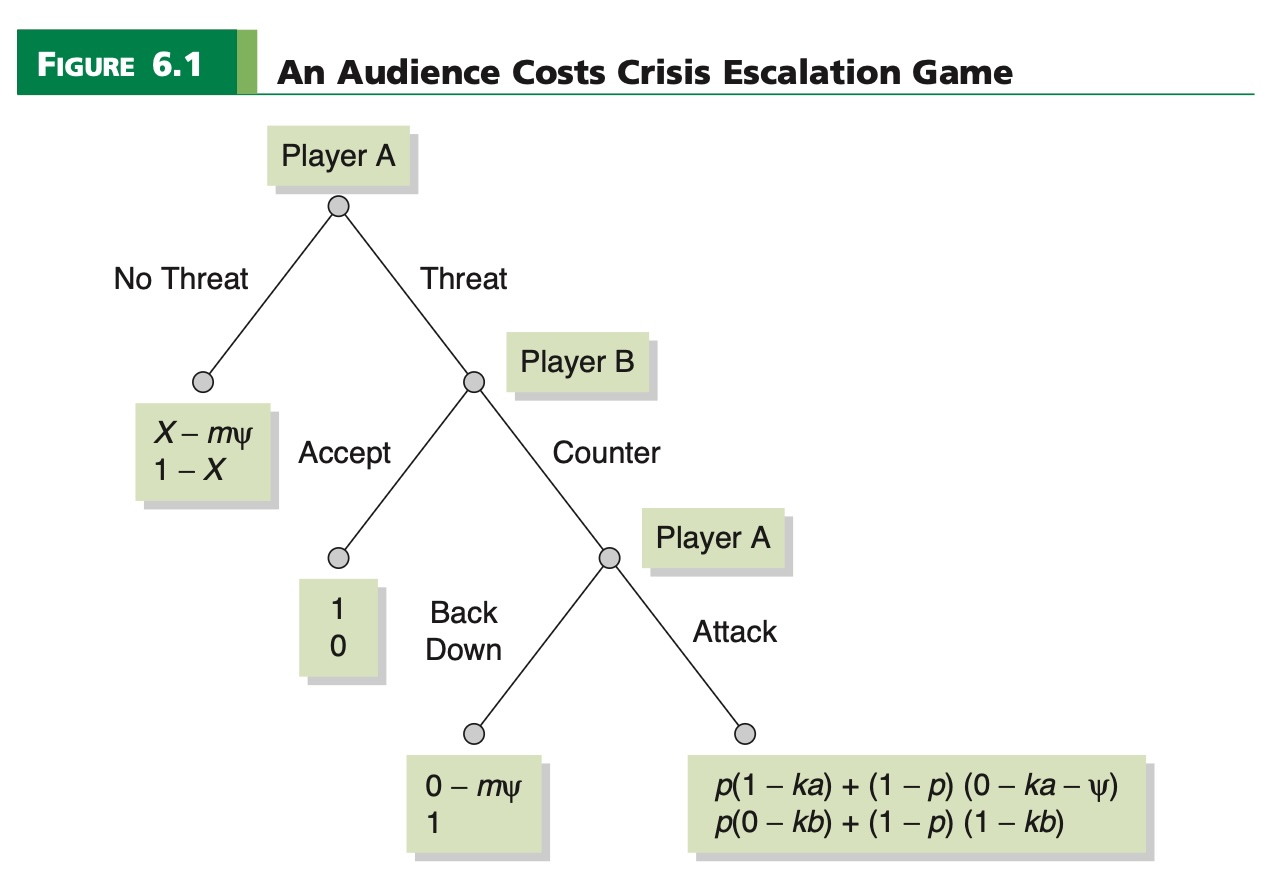
\includegraphics[width=0.7\textwidth]{images/audience_costs_crisis_escalation_game.jpg}
    \captionof{figure}{\label{fig:fig8_audience_costs_crisis_escalation_game.jpg}%\textit{\parencite[Fig.\(\backsim\)1]{cranmerWhatCanWe2017}}
    }
\end{center}

\begin{itemize}
    \item Let $0 \leq m \leq 1$: the variable $m$ measures the degree of domestic policy inadequacy (the general risk of not being reselected) based on prior job performance.

    \item $\Psi$ is the cost to a leader of being turned out of office: a constituency- or audience-imposed cost.

    It measures the audience costs associated with the leader’s choices in the game since loss of office is the cost the selectorate can impose on a leader who fails to deliver the benefits they seek.

    \item $X$ is the value of the status quo to player A.

    \item $p$ is the probability that A wins if A attacks B.

    \item $k_a$ and $k_b$ are A's and B's expected costs from war.

    \item Assumptions: winning a war or making a successful threat ensures remaining in office. Losing a war ensures losing office. Backing down after threatening war or not threatening war implies that the loss of office depends on the degree to which the leader's record is considered inadequate ($m$).
\end{itemize}

% In this game, A’s possible strategies are:
% \begin{enumerate}
%     \item [(1)] threaten and attack;
%     \item [(2)] threaten and back down (bluff)
%     \item [(3)] not threaten and attack: this strategy is eliminated by the rules for calculating a subgame
%     perfect Nash equilibrium
%     \item [(4)] not threaten and back down.
% \end{enumerate}

% In this game, B’s possible strategies are:
% \begin{enumerate}
%     \item [(1)] counter A’s demand
%     \item [(2)] accept A’s demand
% \end{enumerate}

$\Psi\ \text{and}\ m$ are both domestic features in the crisis decision-making game and so \textbf{are not part of a realist perspective}.

\subsubsection{Solving when $\Psi = 0$ and $m = 0$}
Backward induction reveals that A will attack rather than back down if A has threatened and if $p > k_a$.

B can be expected to counter under two circumstances:
\begin{enumerate}
    \item [(1)] if A is expected to back down (B believes $p < k_a$)
    \item [(2)] if B believes A will attack but B believes that $1 - p > k_b = $ B’s expected chance of winning $1 - p >$ B’s expected costs from a war ($k_b$).
\end{enumerate}

A initiates a threat only if:
\[A\ believes\ that\ B\ believes\ 1 - p < k_b\]
\[B\ will\ not\ counter\]
\[A\ believes X + k_a < p\]
\[\text{X is so bad that it is worth gambling on a war}\]

In each instance, we see that:
\[p\ \uparrow\ \Rightarrow\ \uparrow\ Probability\ A\ makes\ a\ threat\]
\[p\ \uparrow\ \Rightarrow\ \uparrow\ \text{threaten and
more likely to fight if B makes a counter demand instead of backing down}\]

\subsubsection{Solving when $\Psi > 0$}
Holding everything else constant, increased audience costs
changes the size of the fraction that $p$ must be larger than in order to attack rather than back
down.

If $m$ is sufficiently large, then the leader of A is prepared to attack even with a small chance of winning as this is its best shot at salvaging his or her reelection prospects.

So good prior policy performance can offset the incentive to attack even when audience costs are high.

We learn from audience costs two important things: each pulling in opposite directions with regard to settling disputes.

\begin{itemize}
    \item that democrats are less likely to make idle threats
    \item democrats might attack even when their chances of victory are low
\end{itemize}

\subsection{Crisis Selection in Democracies and Autocracies}
As Schultz (1998, 2001) has noted, audience costs lead to interesting selection effects in terms of what we actually get to observe in the world.

A legitimate opposition is absent from audience-costs models.

In Schultz’s formulation
\begin{itemize}
    \item because the opposition party is interested in gaining electoral advantage, it opposes foreign policies the incumbent proposes if the opposition deems the policy likely to fail.
    \item When the foreign policy is thought to have a good chance of success, the democratic opposition backs it to minimize the electoral advantage gained by the incumbent’s party.
\end{itemize}

When the opposition supports the incumbent’s foreign policy, this support credibly conveys “high resolve” to the foreign opponent. This has two effects: (1) it encourages the democratic incumbent to press ahead with his foreign policy and (2) it discourages the rival from believing that internal dissension in the democracy will weaken the democratic leader’s resolve to fight.

The audience-costs literature offers an explanation for differences in the crisis behavior of autocrats and democrats. It helps us understand selection effects that shape what we actually observe in the international arena.

\subsection{Diversionary War}
Smith (1996, 1998) developping a model in which audience costs are an endogenous, strategic element of the political environment.

In Smith’s model, leaders can use their private information to manipulate policy, choosing, for instance, diversionary war tactics designed to draw attention away from their previous policy failures (the variable m in the game in figure 6.1). Other models, such as those by Slantchev (2006) and Ashworth and Ramsay (2011) further develop these themes.

In the Ashworth-Ramsay model, for instance, leaders have private information about their nation’s prospects in war (p in figure 6.1). That information can be used to extract a substantial concession from the foreign rival who wishes to avoid the costs of war (kb). But the fact that the initiation of conflict could extract a significant concession to appease the initiator means that the prospective initiator also has incentives to create a crisis when her private information does not support a strong expectation of victory.

Ashworth and Ramsay report that under optimal conditions, citizens always punish leaders if they initiate a crisis and then back down. Whether leaders are punished if they back down rather than going to war, however, depends on the value of the status quo and on the costs of war, much as we saw in the game in figure 6.1.

Gaubatz (1991), Fordham (1998), and Smith (2004), for example, show that war timing by democratic leaders is strongly influenced by where they are in their election cycle, their reelection prospects, and the electoral rules under which they operate.

Conconi, Sahuguet, and Zanardi (2010) show that democratic term limits lift some of the constraints on war fighting that otherwise characterize reelection-motivated choices in democracies.

Morrow focused on arms control negotiations between the United States and the Soviet Union, demonstrating that when the US economy faced high inflation or high unemployment (i.e., m is large in figure 6.1), the president was prepared to grant greater concessions to the powerful Soviet Union in arms control talks to offset his domestic economic shortcomings and to improve the odds of a negotiated resolution of important, contentious foreign policy issues.

Tarar focuses on what makes a diversionary threat into a meaningful signal of leader competence. He argues that the rival must be sufficiently strong that the conflict actually tests competence, and the leader must place a sufficiently high value on retaining office. Tarar’s model helps make sense of seemingly competing empirical patterns.

\subsubsection{The Resurrection Hypothesis - Downs and Rocke (1995)}
When leaders face a military defeat and anticipate being ousted, extreme efforts are actually a rational response.

Such leaders lose nothing by fighting on and stand to gain much if luck should turn their way.

\textbf{Example: Tet Offensive during Vietnam War}
US military and political leaders believed that they had already punished the North Vietnamese regime to such an extent that it was no longer capable of launching a military offensive. Likewise, the American public had become convinced that the war in Vietnam was virtually won. And, in fact, the Tet offensive was a considerable military rout But just by the very fact that they were able to launch the offensive at all, the North Vietnamese pulled off a stunning political and propaganda victory that resurrected their hopes and led, ultimately, to a negotiated resolution of the Vietnam War that was very favorable to the North Vietnamese side.

\textbf{Example: Iraq 2003}
Bluffing about WMD weapons, Saddam might have hoped to convince the opposition in the United States to oppose going to war given the high expected costs in terms of casualties.

Saddam Hussein may have decreased the odds of an invasion by raising the specter of an unconventional war.

When a country demonizes an adversary, this helps mobilize domestic political support for the use of force, thereby increasing the chances of victory against the adversary. However, demonizing an enemy also motivates that adversary to try harder to win.

\subsubsection{Pacific Dove Hypothesis}
There is a hypothesis, known as the pacific dove hypothesis (Bueno de Mesquita and Lalman 1992) that is closely associated with the logic of the resurrection hypothesis.

\textbf{Dove:} prefers to resolve disputes through negotiation rather than trying to coerce an adversary.

\textbf{Pacific Actor: Bueno de Mesquita and Lalman (1992)} if attacked, prefers to surrender.

If a state—or nonstate actor such as a terrorist group— is a pacific dove and if it is uncertain of its foe’s type (dove or hawk, pacific or aggressor), then the weaker the pacific dove is relative to its opponent, the higher the probability that it will launch an attack in an effort to extract a surrender from that opponent.

The logic undergirding this seemingly counterintuitive claim is developed in a model known as the \textbf{international interaction game}.

The international interaction game assumes that there is a first-strike advantage, which might be small or large, and that this \textbf{first-strike advantage can create a commitment problem} that makes efforts to negotiate risky.

Negotiations do not look that attractive to the weak pacific dove because its weakness means it lacks leverage.

Giving up the first-strike advantage and facing the danger of being forced to cave in looks bad too.

For the weak pacific dove the best prospect is to attack and hope that its stronger rival is not motivated to fight back.

This is the only way that a weak pacific dove can derive benefits from the situation.

Bueno de Mesquita and Lalman (1992) tested the pacific dove hypothesis on all European disputes across almost 200 years of history. Although there are just forty instances of pacific doves in that analysis, they found that they behaved as predicted.

That pacific doves are more likely to engage in violence when they are weak rather than strong raises difficult questions about conflict resolution.

\textbf{Both hawks and weak pacific doves (but not powerful pacific doves) behave in the same way when they are sufficiently uncertain of the response they can expect if they pursue peaceful solutions to their disputes.}

\subsection{Selectorate Theory and the Conduct of War}

Small-coalition leaders look for valuable territory to acquire or treasure that they can capture for their own domestic use.

For democratic regimes <wars are directly or indirectly about policy issues. Either they fight to extract concessions or to impose regime change in order to put in power someone who will grant the desired policy concessions.

\textbf{Take Away:} We see that the reasons behind militarized disputes, both those that become wars and those that fall short of open warfare, are different depending on the accountability of the regime to a larger or smaller audience.

\textbf{Selectorate Theory + Audience Cost Model:}
Selectorate theory provides a substantive underpinning that is coalition-dependent behind the reason for fighting: democrats need to provide adequate public goods, including foreign policy concessions from adversaries, in order to stay in office. Autocrats need to provide resources with which to pay off cronies. Otherwise, members of their coalition will switch their loyalty to someone better able to provide private rewards.

This regime-type distinction turns out to have implications for decisions to fight or not and for differences in the effort made to win once war is underway.

\subsubsection{War-Selection Calculations}
Well-established empirical regularity that democrats, with their dependence on a large coalition, tend to win the wars they fight.

Major reason that democrats do so well in war is that they are highly selective about the wars they fight, choosing to negotiate when the odds of victory in war are not substantial.

\subsection{Selectorate Theory and War Effort}
Let's see the logic and the evidence to \textbf{explain the effort democracies make when a war turns out to be harder} to win than expected.

Let's suppose, as before, that we have two countries, $A$ and $B$, either on the verge of war or already at war. For the sake of argument, we will assume that $A$'s leadership depends on a large coalition of backers and that $B$'s does not.

The leaders of both $A$ and $B$ have access to money, such as government revenue, with which to pay for public and private goods. We will call this resource pool $R$. The leader of $A$ can choose to distribute all of $R$, in the limiting case, to the winning coalition or allocate some or all of it to the war effort. Let $R_{\mathrm{coalition}}$ denote the resources distributed to the winning coalition and $R_{\mathrm{war}}$ the resources allocated to the war effort. The budget constraint is

\begin{equation}
    R = R_{\mathrm{coalition}} + R_{\mathrm{war}}.
\end{equation}

In the extreme case, suppose that the leader of $A$ knows that the country can defeat $B$ with certainty if all available revenue is allocated to the war effort:

\begin{equation}
    R_{\mathrm{war}} = R \Rightarrow \Pr(A \text{ defeats } B) = 1.
\end{equation}

Conversely, if no additional resources are allocated to the war effort because $R$ is retained to provide private benefits to key backers, the war will certainly be lost:

\begin{equation}
    R_{\mathrm{war}} = 0 \Rightarrow \Pr(A \text{ defeats } B) = 0.
\end{equation}
\begin{enumerate}
    \item $V$ public good of victory and any other policy gains it implies.
    \item $r$ total value of private benefits that can be extracted from the vanquished state and distributed among the victor's coalition members. $W$ the size of the victor's winning coalition. The private benefit received by each coalition member is $r \slash W$. (we assume that every member of the victor's winning coalition receives an equal share of these private gains).
\end{enumerate}

A victory total value: $V + r/W -k$ ($k$ is the cost of war).

The smaller the leader’s winning coalition the more acceptable it can be to lose a war rather than spend the coalition’s money on victory.

That is, to fight to victory, spending all of R in the process—rather than lose while keeping
R—the following must be true:

\begin{equation}
    V + \frac{r}{W} - k \geq \frac{R}{W} - k
    \quad \Rightarrow \quad
    V \geq \frac{R-r}{W}.
\end{equation}

\textbf{Thus: if A is democratic, A will value victory
relative to keeping revenue much more than will B if B is autocratic.}

\subsubsection{Evidence for the War Effort Logic}
\begin{center}
    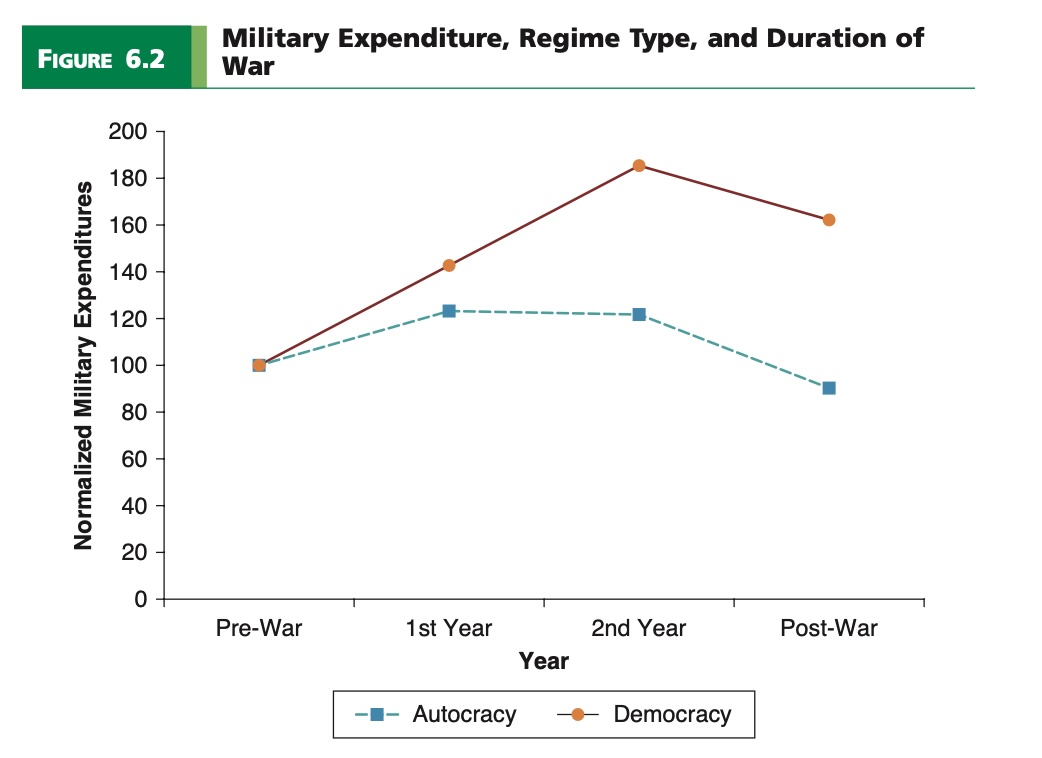
\includegraphics[width=1\textwidth]{images/military_expenditure_regime_type_duration_war.jpg}
    \captionof{figure}{\label{fig:fig9_military_expenditure_regime_type_duration_war.jpg}%\textit{\parencite[Fig.\(\backsim\)1]{cranmerWhatCanWe2017}}
    }
\end{center}

\textbf{This figure shows that democrats facing a prolonged war increase their effort tremendously.}

Figure 6.2 also shows us what happens after the war is over. Democrats cut back modestly on military spending, while autocrats return to their baseline level or even below.
The systematic evidence supports the war effort logic

\subsection{War Effort, War Loss, and Leader Deposition}
Since victorious democrats are more likely to depose and replace vanquished rivals than are victorious autocrats, small-coalition dictators must be especially nervous about defeat at the hands of a democrat.


% Session 05 summaries
% Intended to be included from an existing main.tex.
% No document class, packages, or document environment are defined here.

\section{Allison -- Conceptual Models and the Cuban Missile Crisis}
\subsection{The problem of conceptual lenses}
Allison uses the Cuban Missile Crisis not only as an important historical case but also as a way to investigate how analysts explain governmental behavior. His central claim is methodological: explanations of foreign policy are never produced from facts alone. Analysts approach evidence through implicit \emph{conceptual models} that determine which facts appear important, what counts as a puzzle, which causal mechanisms deserve attention, and what kind of answer will count as an explanation. Different conceptual lenses can therefore generate different explanations of the same event without any change in the underlying historical evidence.

The article advances three general propositions. First, analysts of foreign and military policy normally rely on implicit conceptual models. Second, most conventional analysis is dominated by what Allison calls the \emph{Rational Policy Model} (Model I), in which a national government is treated as a unified actor selecting actions in pursuit of strategic objectives. Third, two alternative perspectives---the \emph{Organizational Process Model} (Model II) and the \emph{Bureaucratic Politics Model} (Model III)---can reveal determinants of governmental behavior that Model I obscures. The three perspectives are illustrated by applying each to the same central question: why did the United States respond to Soviet missiles in Cuba with a naval blockade rather than with another policy?

Allison's chess metaphor captures the difference among the models. Model I imagines a single chess player choosing moves strategically. Model II asks whether apparently coherent moves are instead generated by semi-independent organizations, each operating according to its own routines. Model III asks whether the moves are the result of bargaining among several players who share control over the pieces and pursue partly different objectives. The models thus direct attention respectively toward strategic choice, organizational routines, and political bargaining.

\subsection{Model I: Rational Policy}

Model I treats foreign-policy behavior as \emph{national choice}. The basic actor is a unitary national government with a coherent set of goals, a set of perceived alternatives, and estimates of the consequences of each alternative. A strategic problem creates threats and opportunities, and the government responds by selecting the action whose expected consequences best advance its objectives. The key elements are therefore goals and objectives, available options, expected consequences, and value-maximizing choice.

The model's dominant inference pattern runs backward from observed action to purpose. If a government performed action $X$, the analyst asks what objective would make $X$ a reasonable or optimal means. Explanation consists in reconstructing the rational connection between national objectives and the chosen action. Allison argues that this logic is widespread in international-relations scholarship even when it is not explicitly acknowledged. Different analysts may disagree about national objectives or constraints, but they frequently share the assumption that an important foreign-policy act is a calculated response by a unified state.

The model generates straightforward comparative propositions. If the costs of an option rise, or its probability of success falls, that option should become less likely; if its costs fall or its expected effectiveness rises, it should become more likely. Deterrence theory is a prominent example. A secure second-strike capability raises the expected costs of a nuclear first strike and should therefore reduce its attractiveness to a rational opponent.

Applied to the Cuban Missile Crisis, Model I depicts the blockade as the result of a systematic comparison of alternatives. The United States considered several broad courses of action. Doing nothing was rejected because the missiles were seen as militarily and politically significant and because failure to respond would undermine the credibility of American commitments. Pure diplomatic pressure appeared too slow and might force Washington into politically damaging concessions. A secret approach to Castro could not solve the problem because the missiles were controlled by the Soviet Union. A full invasion promised to remove both the missiles and Castro but risked direct combat with Soviet forces and a wider superpower confrontation. A surgical air strike offered speed but could not reliably destroy all missiles and risked appearing as a surprise attack. The blockade stood between passivity and immediate attack. It demonstrated resolve, exploited U.S. local superiority, slowed further Soviet deployments, and left Moscow time and room to retreat without immediate humiliation. From the Model I perspective, it was a value-maximizing form of limited escalation.

This first cut is powerful because it imposes coherence on the crisis. Yet precisely this coherence is what the other two models question. Governmental action may not be the product of a single calculation, and the options presented to leaders may themselves be shaped by organizational capabilities and political struggles.

\subsection{Model II: Organizational Process}

Model II opens the governmental ``black box.'' A government is not one actor but a conglomerate of large organizations. Leaders formally sit at the top, but most information, planning, preparation, and implementation are performed by organizations that possess established missions, routines, procedures, and repertoires. What Model I calls a national ``choice'' is therefore often better understood as an \emph{organizational output}.

Large organizations are indispensable because governments must monitor many problems and perform complex tasks simultaneously. They divide broad problems into narrower responsibilities and assign them to specialized units. This produces competence and regularity, but it also produces \emph{parochial priorities}. An organization tends to perceive problems through its own mission and capabilities. It develops standard operating procedures (SOPs) that allow ordinary members to handle recurring situations without reconsidering every problem from first principles. Complex actions are implemented through programs that coordinate many routines. Consequently, what leaders can actually order is constrained by the programs already available: governments can usually choose effectively only among actions for which organizations possess some existing capability and repertoire.

Model II therefore emphasizes continuity. The best clue to what an organization will do at time $t$ is often what it was doing at $t-1$. Organizational behavior changes incrementally because routines, budgets, professional norms, equipment, and division of labor cannot be redesigned instantly. Search is generally problem-directed and local: when performance falls below acceptable levels, organizations look first for solutions near existing routines. Learning and change occur, but they are usually gradual and shaped by existing organizational capacities.

This perspective changes the interpretation of the missile crisis. Soviet behavior need not be explained entirely by a single strategic calculation. Details of missile deployment, construction, camouflage, and military procedure may have reflected familiar Soviet organizational routines developed for other contexts and transferred to Cuba. Likewise, American intelligence did not simply ``decide'' when to discover the missiles. Detection depended on organizational procedures, reconnaissance routines, interpretive categories, and the availability of information through established channels.

The blockade itself also illustrates the autonomy of organizational implementation. Presidential leaders could decide on a quarantine in broad terms, but the Navy had to convert that political decision into an operational program. Naval doctrine and established procedures defined how ships would intercept, hail, inspect, and if necessary stop Soviet vessels. The resulting action was not infinitely adjustable to presidential wishes. Allison recounts the tension between Secretary of Defense Robert McNamara and Admiral George Anderson over how the blockade would actually be conducted. When McNamara demanded precise answers about interception procedures, Anderson relied on the Navy's established regulations and insisted that the Navy should run the blockade. The episode illustrates Model II's central point: even at the height of a crisis, implementation reflects organizational routines that political leaders cannot simply rewrite at will.

Model II thus qualifies the rational-choice story. Leaders may choose among broad alternatives, but the menu itself is organizationally generated, information is filtered through organizational channels, and execution is shaped by SOPs. Apparently puzzling details may therefore be explained not by grand strategic objectives but by the mundane fact that an organization did what it already knew how to do.

\subsection{Model III: Bureaucratic Politics}

Model III shifts from organizational routines to political bargaining. The leaders at the top of governmental organizations are not a single team with one objective. They are individual players occupying different positions, carrying different responsibilities, perceptions, interests, and commitments. Governmental action is therefore often a \emph{political resultant}: an outcome produced by ``pulling and hauling'' among players rather than a solution deliberately selected by a unified actor.

The model starts from three conditions. Power is shared among several participants; those participants disagree about what should be done; and the stakes are important enough that they fight to influence the decision. Position matters because responsibilities shape perceptions and priorities. This is summarized in the famous proposition that ``where you stand depends on where you sit.'' Military chiefs, diplomats, intelligence officials, and political advisers confront different organizational demands and therefore tend to define problems differently. The proposition also works vertically. Presidents, cabinet chiefs, senior staff, and lower-level officials face different constraints. Presidents must preserve flexibility and decide among competing claims; chiefs must build coalitions and secure presidential attention; lower-level officials struggle to place issues and proposals on the agenda.

Bureaucratic politics takes place through established \emph{action channels}: regular procedures that determine who participates in which decisions, at what stage, with what information and authority. A player's influence depends not only on formal position but also on bargaining advantages, expertise, control of information or implementation, access to the president, personal skill, willingness to use political resources, and the intensity of the player's preferences. Deadlines and previously made commitments matter because they narrow the space for bargaining and can allow decisions to emerge before every participant has reconsidered all alternatives.

The third cut at the Cuban Missile Crisis explains the blockade as the product of coalition formation inside the Kennedy administration. Important advisers initially favored different options. The Joint Chiefs and several senior figures strongly supported an air strike. McNamara increasingly regarded a blockade as a more controllable alternative. Robert Kennedy objected to a surprise air attack on moral and political grounds, fearing that it would make the United States resemble the perpetrators of Pearl Harbor. Theodore Sorensen also moved toward the blockade. The personal and political relationship of these advisers with President Kennedy mattered, as did the way different options were presented.

A decisive coalition gradually formed around McNamara, Robert Kennedy, and Sorensen. Meanwhile, advocates of an air strike included figures whose style and relationship with the president made their recommendations less persuasive to him. Information also entered the political game. The claim that an air strike could not be reliably ``surgical'' strengthened the blockade coalition, even though Allison notes that some of the information underlying this judgment was inaccurate or insufficiently examined. The final choice therefore cannot be reduced to a neutral ranking of fixed alternatives. It emerged from the timing of meetings, coalition building, personalities, institutional positions, arguments, and the distribution of influence among the players.

Model III also changes the meaning of governmental intention. An outcome can be coherent enough to count as government policy without having been intended in all its details by any one participant. Different actors may contribute different pieces of the final action for different reasons. The result can therefore be distinct from the preferred policy of every individual participant.

\subsection{Overall implications}

Allison does not argue that one model is universally correct and the others false. Rather, each highlights one class of determinants while holding others in the background. Model I emphasizes pressures and incentives in the international strategic environment. Models II and III examine the internal governmental machinery through which those pressures are perceived and converted into action. They are not mutually exclusive, and a fuller theory would need to specify which kinds of decisions are best explained by which mechanisms and how the mechanisms interact.

The broader lesson is a demand for analytical self-consciousness. Researchers should identify the assumptions embedded in their explanations rather than treating one conceptual lens as natural or neutral. The same event can look like a rational choice, an organizational output, or a political resultant depending on the model used. Models II and III are particularly useful as correctives to the tendency to infer large purposes from large events. They can improve explanation and prediction by directing attention to organizational capabilities, routines, intra-governmental disagreement, and bargaining.

At the same time, Allison recognizes limitations. Model I can rationalize almost any observed action if objectives are freely reconstructed. Model II risks explaining the present too heavily by the past and needs a better account of organizational change. Model III can become extremely complex and informationally demanding. The article therefore ends with a research agenda rather than a finished synthesis: foreign-policy analysis should make its conceptual models explicit, derive propositions more systematically, and combine strategic, organizational, and political variables in ways that improve both explanation and prediction.

\clearpage
\section{Jonathan Bendor and Thomas H. Hammond --- \emph{Rethinking Allison's Models}}

\subsection{Purpose and general critique}

Bendor and Hammond revisit Graham Allison's \emph{Essence of Decision} more than two decades after its publication. They acknowledge its enormous contribution: Allison showed how explicit models could generate alternative explanations of the same foreign-policy event and helped move the study of bureaucracy away from purely descriptive accounts. Their concern, however, is that the three famous models---rational actor, organizational process, and governmental politics---are less internally coherent than their influence suggests. The article therefore evaluates the models primarily as theories rather than reassessing the historical record of the Cuban Missile Crisis.

They develop five broad criticisms. First, the assumptions underlying Allison's models are often unclear. Second, many propositions are not logically derived from those assumptions. Third, some important propositions, especially in Model II, are logically wrong. Fourth, the models do not strike an appropriate balance between simplicity and complexity: Model I is too thin, whereas Model III is too thick. Fifth, Allison sometimes misrepresents the intellectual traditions from which the models are supposedly drawn. This matters because many readers have used \emph{Essence of Decision} as an introduction to rational choice, organization theory, and bureaucratic politics.

\subsection{A typology of policymaking models}

To clarify the problem, Bendor and Hammond construct a typology based on four dimensions: the number of decision makers, whether multiple actors have common or conflicting goals, whether actors are perfectly or imperfectly rational, and whether information is complete or incomplete. The typology demonstrates that Allison's models combine several dimensions at once, making it hard to know which assumption drives a particular prediction.

Model I appears to assume a single, perfectly rational actor, often with complete information. Models II and III are harder to classify. Model II is associated with bounded rationality and organizational routines, but Allison also introduces conflicting organizational goals. Model III clearly contains multiple actors with conflicting goals, yet it is ambiguous about whether those actors are fully rational or boundedly rational. It also incorporates misperception, incomplete information, bargaining, foul-ups, and incrementalism. As a result, Models II and III overlap analytically more than Allison's presentation implies. Before combining them, the authors argue, one should clarify exactly what each assumes.

\subsection{Model I: an unfairly weak version of rational choice}

Bendor and Hammond argue that Allison's Model I is not a fair test of rational-actor analysis because it is an unnecessarily primitive version of rational choice. Rationality does not require a single goal. An actor can pursue multiple, even competing objectives so long as preferences are consistently ordered. In the Soviet decision to deploy missiles in Cuba, for example, concern with the strategic nuclear balance could have coexisted with goals such as defending Cuba or reducing U.S. prestige. Showing that missile deployment was not optimal for every subsidiary goal does not prove those goals were irrelevant.

The model is also excessively static. Allison's rational actor chooses once at a single moment, whereas real foreign-policy decisions have consequences across time. A proper rational model can incorporate intertemporal trade-offs and discounting. Likewise, Model I largely neglects uncertainty. Rational-choice theory can analyze risk, imperfect knowledge of external events, and uncertainty about the preferences or capabilities of other states. Actors may be risk-averse, risk-neutral, or risk-seeking, and these attitudes affect choice.

Most importantly, Allison neglects strategic interaction. In international relations, the strongest justification for treating states as unitary rational actors is precisely that doing so allows the analyst to study strategic relations among states. Yet Allison's formal statement of Model I resembles individual decision theory, in which an isolated actor selects the best option from a fixed menu. Crisis bargaining is instead a game: each state's optimal action depends on the expected response of the other. Concepts such as Nash equilibrium, multiple equilibria, Pareto-inferior equilibria, and mixed strategies demonstrate that rationality does not imply a simple mapping from preferences to outcomes. A Prisoner's Dilemma can produce an outcome both sides dislike, while Chicken can contain multiple equilibria with very different distributions of gains. Strategic uncertainty can arise even when actors know the structure of the game.

The authors therefore reject the common lesson that the Cuban crisis proves the weakness of unitary rational-actor explanations. Allison's particular version of Model I was so underdeveloped that it should have been expected to perform poorly. A richer rational-choice model, especially one incorporating game theory and incomplete information, could generate much more powerful explanations.

\subsection{Model II: routines do not necessarily imply simple behavior}

Bendor and Hammond regard Allison's treatment of organizational routines as pioneering but criticize his interpretation of bounded rationality. Allison moves from the plausible claim that individuals use simple decision rules and SOPs to the stronger claim that organizational behavior will therefore be simple, rigid, incremental, and predictable. The authors argue that this inference is invalid. Complex behavior can emerge from simple rules, especially when many rules interact. Even a single adaptive decision maker using simple heuristics can produce complicated patterns, and an organization can combine many specialized routines into sophisticated behavior.

Allison also underestimates the positive functions of organizations. Simon and March did not view routines merely as constraints. Division of labor, specialization, redundancy, and organizational procedures can compensate for the cognitive limitations of individuals. Organizations can process more information and perform more complex tasks than any single member. SOPs can therefore \emph{enable} action as well as constrain it. Whether routines improve or degrade performance depends on the environment and on how well the routines match the problems faced.

The proposition that organizational behavior at $t+1$ will be only marginally different from behavior at $t$ is consequently too strong. Stable routines can generate nonlinear or surprising aggregate outputs, and organizations can recombine elementary programs in novel ways. The important theoretical question is not simply whether routines exist---all organizations require them---but how particular structures, procedures, information systems, and adaptation mechanisms shape performance.

\subsection{Model III: bargaining, hierarchy, and excessive complexity}

The authors' central criticism of Model III is that Allison treats bargaining as pervasive without explaining when superiors actually need to bargain with subordinates. The president possesses formal authority, appoints senior officials, and can in principle dismiss them. Why, then, must policy always be the result of bargaining among quasi-independent players? Bureaucratic-politics theory should identify the conditions under which hierarchy fails to produce command and bargaining becomes necessary.

Bendor and Hammond identify two especially important sources of subordinate influence. First, subordinates may possess political support outside the executive branch---in Congress, interest groups, professional communities, or other constituencies---which makes it costly for the president to override them. Second, subordinates may enjoy informational or technical advantages. They can influence which problems reach the president, which options are presented, and how decisions are implemented. Yet these advantages are variable. Presidential attention, alternative information channels, clear preferences, and control over appointments can reduce subordinate power. Bureaucratic politics should therefore be treated as conditional rather than universal.

Hierarchy itself is insufficiently theorized in Allison's Model III. Organizational structure determines who communicates with whom, which comparisons are made, which issues reach senior decision makers, and in what sequence alternatives are evaluated. Different hierarchies can therefore produce different policies even with identical actors and preferences. The interaction between formal authority and specialized expertise is a central feature of bureaucracy, but Allison does not develop it systematically.

The famous proposition that ``where you stand depends on where you sit'' also has ambiguous theoretical status. Position can influence preferences, but individuals are not reducible to their offices, and the proposition needs conditions and mechanisms if it is to be testable. More broadly, many Model III propositions are not clearly deduced from the model's premises.

Finally, Model III includes so many variables---positions, personalities, perceptions, bargaining advantages, organizational interests, deadlines, coalitions, personal commitments, and much more---that it risks becoming an ``analytical kitchen sink.'' A useful model must simplify. If a theory contains almost every potentially relevant feature of a case, it may describe events richly but cannot generate clear, falsifiable predictions. The authors suggest concentrating on a smaller number of structural variables, especially hierarchy, authority, expertise, informational asymmetry, and external political support.

\subsection{Conclusion}

Bendor and Hammond preserve Allison's methodological achievement while rejecting the theoretical authority often granted to his specific models. \emph{Essence of Decision} taught scholars to formulate explicit alternatives and to ask how different assumptions produce different explanations. That remains valuable. But the actual models require substantial reformulation.

Their final assessment is fivefold. Allison's models do not accurately represent all the literatures on which they are based; Model I does not give rational choice a fair test; the assumptions separating Models II and III are ambiguous; important propositions are not rigorously derived, and some are incorrect; and empirical support for a proposition teaches little about a model if the proposition is not logically connected to that model. Advances after 1971 make some weaknesses more visible, but many problems were present from the beginning. The article therefore calls for models that are explicit enough to reveal their assumptions, simple enough to yield deductions, rich enough to capture relevant strategic and organizational processes, and precise enough to be tested.

\clearpage
\section{Bruce Bueno de Mesquita and Alastair Smith --- \emph{Domestic Explanations of International Relations}}

\subsection{From unitary states to political leaders and institutions}

Bueno de Mesquita and Smith review the growth of research linking domestic politics to international relations. Their central claim is that foreign policy cannot be adequately understood by treating states as unitary actors with a single national interest. Leaders, advisers, supporters, opposition groups, and citizens may have different preferences, and political institutions determine whose interests matter for policy. The modern linkage literature therefore explains international behavior by examining leaders' incentives for political survival, principal-agent problems, domestic accountability, and institutional variation across regimes.

The political-economy approach assumes that leaders generally want to remain in office. They may promote national welfare when doing so supports that goal, but leader and citizen interests can diverge. The relevant domestic constituency varies across systems: in a democracy it may be a broad electorate, while in an autocracy it may consist of a small group of generals, party officials, clans, or cronies. Foreign policy must therefore be incentive-compatible with the political requirements leaders face at home. This perspective connects domestic institutions to war, crisis bargaining, nation building, foreign aid, and economic sanctions.

\subsection{Audience costs and international disputes}

A major strand of the literature examines \emph{audience costs}: domestic political penalties that leaders may suffer if they publicly escalate a dispute and then back down. Fearon's model argues that these costs are higher for democratic leaders because they are accountable to broad constituencies. Public threats can therefore ``tie the hands'' of democratic leaders and signal resolve more credibly. The implication is not simply that democracies are more belligerent. Rather, democratic leaders should be more selective about which crises they enter and which threats they make. If they do issue a threat, opponents may be more likely to believe it.

Later work endogenizes audience costs rather than assuming them. Smith links them to voters' uncertainty about leader competence and to reelection incentives. Slantchev shows that audience costs need not rise monotonically with democracy. Ashworth and Ramsay frame the problem in terms of moral hazard, asking how citizens optimally constrain leaders who may bluff to extract concessions. Schultz adds a domestic opposition party: because an opposition can criticize weak foreign-policy initiatives, its support or silence can itself convey information about the government's resolve. Across these models, the important point is that domestic institutions affect both which disputes are selected into observation and how signals are interpreted internationally.

\subsection{The democratic peace}

The most famous empirical regularity associated with domestic institutions is that democracies rarely fight wars against one another. The article reviews several explanations. Normative theories argue that democracies internalize habits of compromise and extend them to relations with other democracies. Institutional theories instead focus on incentives and selection effects.

Selectorate theory explains foreign policy through the size of the \emph{winning coalition}, the group whose support is necessary for a leader to remain in power, and the broader selectorate from which that coalition is drawn. Leaders dependent on large coalitions must provide relatively broad public benefits, including successful foreign policy. Defeat in war is therefore especially dangerous to democratic leaders. They become highly selective, fighting mainly when prospects of victory are strong, and once at war they have incentives to commit substantial resources to winning. Autocrats, whose survival may depend on a smaller coalition rewarded with private benefits, can tolerate policy failure more easily if they preserve resources for key supporters.

This logic helps explain why democracies are unattractive targets for other democracies. Both sides would need high confidence of victory, a condition that is difficult for two opponents to hold simultaneously. Democracies therefore tend to negotiate rather than fight one another, even though democracies are not inherently pacifist and may fight autocracies or weaker opponents. The review also discusses competing arguments involving issue salience, capitalism, leader experience, and the personal consequences of losing office. The larger lesson is that regime type shapes conflict through specific institutional incentives rather than through an undifferentiated ``national interest.''

\subsection{Diversionary conflict}

Domestic political weakness can also affect the timing and form of foreign policy. Diversionary-war arguments propose that leaders may initiate international confrontations to improve domestic standing. Research shows that election cycles, reelection prospects, term limits, and economic conditions can alter incentives for international action. Yet poor domestic conditions do not mechanically cause war. A politically vulnerable leader may instead make concessions in negotiations if an international agreement can generate political benefits at home, while foreign opponents may strategically accommodate a vulnerable but powerful state to avoid being targeted.

Models centered on leader competence clarify these mixed findings. International conflict can serve as a signal of competence only under certain conditions, for example when the opponent is strong enough that success is informative and when the incumbent values remaining in office sufficiently. The domestic-international linkage therefore produces conditional predictions rather than a simple claim that unpopular leaders start wars.

\subsection{Nation building and foreign aid}

The domestic perspective generates pessimistic expectations about externally imposed democratization. Democratic interveners are accountable to their own constituents and therefore seek foreign policy outcomes those constituents value. If the preferences of citizens in the target state conflict with the intervener's preferred policies, installing a fully accountable democracy can undermine the intervener's objectives. A dependent autocratic regime may be easier to influence because its leader needs to satisfy only a small coalition and can exchange policy concessions for resources used to reward supporters.

This logic also explains patterns of foreign aid. Aid involves donor leaders, donor constituents, recipient leaders, and recipient citizens. Donor governments provide aid when the foreign-policy concessions they can purchase are worth more politically than alternative domestic uses of the resources. Autocratic recipients are often attractive bargaining partners because they can trade policies for resources without needing broad domestic approval. Aid can therefore enhance the survival of autocrats and may do little for ordinary citizens. The literature reviewed by the authors finds strong connections between strategic interests, aid allocations, voting in international organizations, and access to IMF or World Bank resources. In this framework, aid is often better understood as a tool for buying policy compliance than as an instrument designed primarily for development.

\subsection{Economic sanctions}

The sanctions literature illustrates the importance of strategic selection. Simply asking how often imposed sanctions ``work'' is misleading. If a threatened sanction would be sufficiently painful, the target may concede before sanctions are imposed; the most effective sanctions therefore disappear from datasets of actual sanctions. Conversely, governments may impose weak sanctions that they know are unlikely to compel because imposing them yields domestic political benefits, such as appearing firm or satisfying interest groups.

Domestic institutions also affect the political consequences of sanctions. Leaders are not equally vulnerable to economic pain, because different regimes distribute costs differently and leaders depend on different constituencies. Sanctions may destabilize some leaders while allowing others to shift costs onto politically irrelevant groups. Their effectiveness therefore depends not only on aggregate economic damage but also on how that damage affects the coalition essential to the target leader's survival and on the sender's own domestic incentives.

\subsection{Conclusion}

The review concludes that the domestic-politics research program has substantially improved explanations of international behavior. Its key contribution is to replace the fiction of a homogeneous state with models of self-interested leaders operating under institutional constraints and interacting with supporters, opponents, and foreign actors. Audience costs, selectorate institutions, electoral incentives, political survival, and principal-agent problems help explain patterns that unitary-actor theories either miss or treat as exogenous. The authors therefore reject the idea that international relations constitute a separate realm of ``high politics.'' Foreign policy is made by political leaders, and domestic institutions systematically shape both their choices and the international consequences of those choices.

\clearpage
\section{Robert D. Putnam --- \emph{Diplomacy and Domestic Politics: The Logic of Two-Level Games}}

\subsection{Domestic-international entanglement}

Putnam's starting point is that domestic politics and international relations are mutually entangled. Asking whether domestic politics determines international relations or the international system determines domestic politics is therefore misguided; both causal directions operate under different conditions. The theoretical challenge is to explain when and how they interact. Putnam develops the metaphor of the \emph{two-level game} to show how national leaders must negotiate simultaneously with foreign counterparts and with domestic constituencies.

The 1978 Bonn economic summit provides the motivating example. The United States sought more expansionary policies from Germany and Japan, while Germany and Japan pressed the United States to address inflation, the dollar, and energy consumption. The summit produced a broad package: Germany accepted additional fiscal stimulus, Japan promised stronger growth and import expansion, and the United States committed to oil-price decontrol and other measures. Putnam argues that these changes cannot be explained either as pure responses to international pressure or as purely domestic choices. In each country, important domestic factions already favored policies demanded from abroad but lacked sufficient power to enact them alone. International pressure strengthened those factions, while domestic divisions made international concessions politically possible. The agreement succeeded because pressures at the two levels reinforced one another.

This example exposes the limits of both the ``Second Image,'' in which domestic politics causes international behavior, and the ``Second Image Reversed,'' in which international pressures cause domestic outcomes. Both are partial-equilibrium approaches. Putnam instead seeks a framework in which domestic and international bargaining are analyzed simultaneously.

\subsection{The two-level game}

At \emph{Level I}, national negotiators bargain with one another over an international agreement. At \emph{Level II}, domestic groups, parties, legislators, bureaucracies, and other constituents decide whether the agreement is politically acceptable and, where necessary, formally ratify it. The distinction is analytical rather than strictly chronological. Domestic bargaining shapes the mandate and constraints of international negotiators before and during Level I, while expectations about international bargaining affect domestic coalitions. Negotiations may move repeatedly between the two levels.

The chief negotiator sits at both tables. Internationally, the leader seeks an agreement with foreign counterparts. Domestically, the same leader must maintain a coalition capable of accepting or ratifying that agreement. A move that is attractive at one table may be costly at the other. A generous international concession may facilitate agreement abroad but provoke domestic defeat; a hard domestic position may preserve political support but make Level I agreement impossible. Skilled negotiators can sometimes use pressure at one level to change coalitions at the other.

Putnam distinguishes \emph{voluntary} from \emph{involuntary defection}. Voluntary defection occurs when an actor knowingly violates an agreement it could have honored. Involuntary defection occurs when a negotiator genuinely supports an agreement but cannot obtain domestic ratification or implementation. International cooperation therefore depends not only on whether governments reach bargains but also on whether those bargains fall within the domestic political limits of all participants.

\subsection{Win-sets and ratification}

The core concept is the \emph{win-set}. For a given country, the Level II win-set is the set of all possible Level I agreements that would obtain the necessary domestic approval. International agreement is possible only where the win-sets of the negotiating states overlap.

Win-set size has two crucial effects. First, larger win-sets make international agreement more likely because they increase the range of deals that can be ratified on both sides. Small win-sets raise the risk of involuntary defection and can produce bargaining breakdown if there is no overlap. Second, however, a small win-set can create international bargaining power. A negotiator may credibly say, ``I would like to concede, but my domestic constituents will not accept it.'' If the other side wants an agreement, it may have to move closer to the constrained negotiator's preferred outcome. This produces a paradox: domestic weakness can become international strength.

The advantage has limits. Shrinking a win-set may improve a state's bargaining position while overlap remains, but if the win-set becomes too small, the feasible bargaining range disappears and no agreement can be ratified. Putnam's diagram of two contracting win-sets illustrates this trade-off: moderate domestic constraints can improve distributional outcomes, while excessive constraints create deadlock.

Perceptions of win-sets are also strategically important. Negotiators may exaggerate domestic opposition in order to resist concessions, while foreign governments try to estimate which claims about domestic constraints are genuine. Uncertainty about the opposing win-set can generate tactical opportunities but also increase the risk of failed ratification.

\subsection{Determinants of win-set size: preferences and coalitions}

Putnam identifies three broad determinants of win-set size: Level II preferences and coalitions, Level II political institutions, and Level I negotiating strategies.

The first concerns the distribution of domestic preferences. If the costs of no agreement are low for important domestic groups, those groups will demand more from an international bargain and the win-set will be smaller. If no agreement would be very costly, more domestic actors will accept compromise and the win-set expands. The political meaning of ``no agreement'' therefore matters as much as the substantive terms of a proposed deal.

Domestic preference patterns can take different forms. On some issues, interests are relatively homogeneous and actors mainly disagree over how much to demand from abroad: there are domestic ``hawks'' and ``doves.'' On other issues, interests are heterogeneous, so different groups care about different components of a package. Heterogeneity can actually facilitate international cooperation because negotiators can construct packages that combine gains and losses across issues. A policy unacceptable as a single issue may become ratifiable when linked to another issue that benefits the opposing domestic coalition.

This possibility produces \emph{synergistic linkage}. International negotiations can alter domestic coalitions by bundling issues in new ways. Such linkage differs from simple bargaining tricks because the package changes the political feasibility of policies at Level II. The Bonn summit worked partly through this mechanism: international commitments supplied domestic factions with leverage and allowed governments to present a broader package of reciprocal concessions.

The relative political power of domestic groups also matters. Groups that are more organized, intense, or institutionally privileged may constrain ratification disproportionately. Because the composition of the active constituency differs across issues, a country's win-set is not a fixed national characteristic. It varies with the distribution of domestic costs and benefits associated with each negotiation.

\subsection{Domestic institutions and ratification rules}

The second determinant is political institutions. Formal ratification requirements can directly change win-set size. Requiring a simple majority generally creates a larger win-set than requiring a two-thirds majority or unanimity. Stronger ratification hurdles can therefore strengthen a negotiator's international bargaining position but also increase the chance that no agreement will survive Level II.

Informal institutions are equally important. Party discipline, coalition rules, legislative procedures, bureaucratic authority, and traditions of consensus shape what leaders can plausibly deliver. Strong party discipline can expand a leader's win-set by making legislative approval easier. Conversely, systems requiring broad consensus can narrow it.

Putnam uses this logic to reinterpret ``state strength.'' A state whose central executive is insulated from domestic pressure has a large win-set because the leader can ratify many agreements. That autonomy facilitates international cooperation, but it can weaken bargaining leverage: the executive cannot credibly claim that domestic actors prevent it from making concessions. A politically constrained negotiator may have less freedom at home but greater power at the international table. Institutional strength is therefore not unambiguously advantageous.

Real negotiations may involve more than two levels. An international agreement can require approval by a national legislature, parties within a coalition, administrative agencies, regional governments, or organized interests. In the European Community, for example, international decisions can pass through several nested levels of ratification. Each additional veto point changes the effective win-set and complicates bargaining.

\subsection{Level I strategies: changing the other side's win-set}

The third determinant concerns strategies used by international negotiators. A negotiator does not merely observe the foreign win-set; he or she may try to alter it. Side-payments, issue linkage, threats, symbolic gestures, and selective concessions can be targeted at politically pivotal groups in the other country. Successful diplomacy therefore requires knowledge of the opponent's domestic politics.

A concession with little value to the foreign government in the abstract may be crucial if it helps that government assemble a ratifying coalition. Conversely, a threat that imposes costs on politically marginal groups may have little effect, while a smaller but carefully targeted cost can transform the opponent's Level II balance. International bargaining power depends on the domestic incidence of external actions, not merely on their aggregate national effect.

This creates the possibility of transnational alliances. A foreign negotiator may effectively cooperate with domestic groups inside the other state that favor the same international agreement. Such alliances need not be formal. International pressure can supply arguments and resources to domestic minorities, while domestic actors may actively invite foreign pressure to strengthen their own position.

\subsection{Reverberation}

Putnam calls the effect of international pressure on domestic preferences and coalitions \emph{reverberation}. Foreign demands do not simply constrain a fixed domestic game; they can change it. At Bonn, external pressure strengthened domestic supporters of fiscal expansion in Germany and Japan and supporters of energy reform in the United States. International negotiation changed the domestic definition of what was politically feasible and, in some cases, what actors believed to be desirable.

Reverberation can be material or cognitive. Materially, international offers or threats can alter domestic costs and benefits. Cognitively, information and arguments from foreign governments or international institutions can persuade undecided actors, legitimize a policy, or strengthen a domestic minority. Positive reverberation expands the win-set and facilitates cooperation. Negative reverberation produces backlash and shrinks the win-set, especially when pressure comes from a distrusted adversary.

The concept is theoretically important because it prevents analysts from modeling domestic and international politics as independent sequential games. If international strategies can reshape domestic preferences, then Level II outcomes are not exogenous inputs into Level I bargaining. The two levels are genuinely interconnected.

\subsection{The role of the chief negotiator}

For analytical simplicity, the basic model initially treats the chief negotiator as an honest representative of domestic constituents. Putnam then relaxes this assumption. Leaders have their own preferences, political ambitions, reputations, and investments in domestic coalitions. The principal-agent relationship between leaders and constituents therefore matters.

A negotiator may value an international agreement because it enhances domestic political standing, may oppose an agreement that would disrupt an existing support coalition, or may hold personal policy preferences that differ from the median domestic actor. The leader also normally possesses an effective veto: even an agreement that could be ratified may never be submitted if the negotiator dislikes it. Woodrow Wilson's refusal to accept reservations to the League of Nations treaty illustrates how a leader can block an agreement that might otherwise lie within the domestic win-set.

Existing domestic coalitions create ``fixed investments.'' A deal that requires a leader to abandon core supporters and construct a new coalition can be politically costly even if a theoretical majority exists for ratification. Consequently, simple median-voter models may misrepresent the constraints facing actual negotiators. The identity and coalition of the leader matter.

The gap between leader and constituent preferences also creates additional international leverage. If foreign negotiators know that domestic constituents strongly favor an agreement while the leader is reluctant, they may exploit the leader's vulnerability. Conversely, a domestically weak leader facing hard-line constituents may gain bargaining power by credibly claiming that only a favorable agreement can survive politically.

\subsection{Conclusion}

Putnam's two-level framework integrates domestic and international politics without reducing one to the other. It recognizes that ``national interests'' are contested domestically and that national leaders must reconcile international bargains with domestic political survival and ratification. This produces strategic opportunities and dilemmas absent from unitary-actor models.

The framework highlights several recurring mechanisms: voluntary versus involuntary defection; the role of homogeneous and heterogeneous domestic interests; synergistic issue linkage; the paradox that domestic institutional weakness can strengthen international bargaining leverage; targeted threats, concessions, and side-payments; strategic uncertainty about win-sets; reverberation across levels; and conflicts between the chief negotiator's interests and those of domestic constituents.

The broader implication is that successful diplomacy is often not a matter of finding a compromise between two fixed national preferences. It involves constructing agreements that are simultaneously viable in several political arenas. International negotiators bargain not only with one another but also, indirectly, with each other's domestic coalitions. Because the size and composition of win-sets can be changed by institutions, strategies, information, and issue linkage, domestic politics is part of the bargaining process itself. Putnam therefore presents two-level games as a general research framework for explaining both international cooperation and bargaining failure and calls for systematic empirical work to develop and test its propositions.


%------- Bibliography -------
\newpage
\subsection*{\Large Bibliography}
\printbibliography[type=book, title={\large Books}]
\printbibliography[type=article, title={\large Articles}]


%------- Additional Material -------
% \newpage
% \begin{refsection}
%     \nocite{*}
%     \printbibliography[title={\Large Additional Material}, notcategory=cited]
% \end{refsection}

\end{document}
